% **************************************************************************************************************
% Style for the technical report series of the Technische Universität Dortmund
% Based on: A Classic Thesis Style Copyright (C) 2007 André Miede http://www.miede.de
% Adapted by Patrick Krümpelmann 2009
% **************************************************************************************************************

%\documentclass[twoside,openright,titlepage,fleqn,
\documentclass[twoside,titlepage,fleqn,
                pointlessnumbers,headinclude,BCOR5mm,
                ]{scrreprt}

\KOMAoptions{
    paper=a4,
    fontsize=10pt,
%    cleardoublepage=empty,
    footinclude=true
}

\listfiles

%\usepackage{doxygen}

\newcommand{\inst}[1]{$^#1$}
% Variables for the Technical Reports
\newcommand{\myTitle}{A Unifying Response Time Analysis Framework for Dynamic Self-Suspending Tasks }
\newcommand{\myFormattedTitle}{\myTitle}
\newcommand{\myName}{Jian-Jia Chen\inst{1}, Geoffrey Nelissen\inst{2}, Wen-Hung
  Huang\inst{1}}
\newcommand{\myUrl}{\url{http://ls12-www.cs.tu-dortmund.de}}
\newcommand{\myProjectUrl}{~}
\newcommand{\myChair}{$^1$Computer Science 12 at TU Dortmund
  University, Germany\xspace\\
$^2$CISTER/INESC-TEC, ISEP, Polytechnic Institute of Porto, Portugal
}
\newcommand{\myTime}{May 2016\xspace}
\newcommand{\myVolume}{850}

% static for technical reports of the TU Dortmund
\newcommand{\myFaculty}{Department of Computer Science\xspace}
\newcommand{\myUni}{\protect{Dortmund University of Technology}\xspace}
\newcommand{\myLocation}{Dortmund\xspace}
\newcommand{\myDegree}{Technical Report\xspace}
%*******************************************************
\input{classicthesis-config}
%*******************************************************

\usepackage{footnote}
\makesavenoteenv[tablefootnotesave]{table}

%======================================================================================================
% Macros and environments
%======================================================================================================
\usepackage[geometry]{ifsym}
\usepackage{makeidx}
\usepackage{mathrsfs}

\usepackage[T1]{fontenc}
\usepackage{amssymb}
\usepackage{amsmath}
\usepackage{paralist}

\lstset{mathescape=true}
\renewcommand{\theequation}{\arabic{equation}}
\renewcommand{\L}{\ensuremath{\mathbf{L}_{\C,\X,\XL}}}

\usepackage{multido}
%\usepackage[justification=Centering]{subfig}
 \usepackage{tikz}
\usepackage{multirow}
\usetikzlibrary{shadows,patterns,shapes,arrows,decorations.pathmorphing,backgrounds,positioning,fit,plotmarks}

\newcounter{ccount}
\newenvironment{closeenum}
    {\begin{list}{\arabic{ccount}.}
    {\usecounter{ccount}\setlength{\itemsep}{-0.3\baselineskip}
     \setlength{\topsep}{0.15\baselineskip}
     \setlength{\parskip}{0pt}}}
    {\end{list}}

\usepackage{url}
\usepackage{algorithm}
\usepackage{algorithmic}

\newcommand{\ceiling}[1]{\left\lceil{#1}\right\rceil}
\newcommand{\floor}[1]{\left\lfloor{#1}\right\rfloor}
\newcommand{\setof}[1]{\left\{{#1}\right\}}
\newcommand{\set}[2]{\{{#1}\mid{#2}\}}
\newcommand{\equals}{\stackrel{\mathrm{def}}{=}}


\floatname{algorithm}{Algorithm}
\newcommand{\algorithmicinput}{\textbf{Input:}}
\newcommand{\INPUT}{\item[\algorithmicinput]}
\newcommand{\algorithmicoutput}{\textbf{Output:}}
\newcommand{\OUTPUT}{\item[\algorithmicoutput]}
\newcommand{\algorithmicprocedure}{\hskip0.2in \textbf{Procedure:}}
\newcommand{\PROCEDURE}{\item[\algorithmicprocedure]}

%%%%%%%%%%%%%%%
 \def\myendproof{{\ \vbox{\hrule\hbox{%
   \vrule height1.3ex\hskip0.8ex\vrule}\hrule }}\par}
 \newenvironment{proof}{\noindent{\bf Proof. }}{\myendproof}
%%%%%%%%%%%%%%
%%%%%%%%%%%%%%%
 \newenvironment{appProof}[1]{\noindent{\bf Proof of
     #1. }}{\myendproof\vskip 0.1in}
 %%%%%%%%%%%%%%

\newtheorem{theorem}{Theorem}
\newtheorem{Lemma}{Lemma}
\newtheorem{Corollary}{Corollary}
\newtheorem{example}{Example}
\newtheorem{claim}{Claim}
\newtheorem{definition}{Definition}
\newtheorem{rrule}{Rule}
\newtheorem{remark}{Remark}
\newtheorem{observation}{Observation}
\newtheorem{Property}{Property}
\usepackage{etoolbox}
\addtolength{\textheight}{20pt}

\usetikzlibrary{%
  arrows,%
  shapes.misc,% wg. rounded rectangle
  shapes.arrows,%
  chains,%
  matrix,%
  positioning,% wg. " of "
  scopes,%
  decorations.pathmorphing,% /pgf/decoration/random steps | erste Graphik
  shadows%
}

\pgfdeclarelayer{background}
\pgfdeclarelayer{foreground}
\pgfsetlayers{background,main,foreground}
\tikzstyle{materia}=[draw, fill=white, text width=1.0em, text centered,
  minimum height=4em,drop shadow]
\tikzstyle{practica} = [materia, text width=18em, minimum width=8em,
align =left,
  minimum height=3em, rounded corners, drop shadow]
\tikzstyle{texto} = [above, text width=6em, text centered]
\tikzstyle{linepart} = [draw, thick, color=blue!50, -latex', dashed]
\tikzstyle{line} = [draw, line width = 2pt, color=blue!50, -latex']
\tikzstyle{ur}=[draw, text centered, minimum height=0.01em]


\newcommand{\citetechreport}[1]{\ifbool{techreport}{}{ in the report \cite{ecrts16-techreport}}}

\usepackage{pgfplots}

\def\deltasum{\delta_{\mbox{sum}}}
\def\musum{\mu_{\mbox{sum}}}
\def\deltamax{\delta_{\max}}
\def\mumax{\mu_{\max}}
\addtolength{\textheight}{6pt}

\newif\ifpaper
\newif\iftechreport
\newif\iftutechreport
\papertrue 
\techreporttrue
\tutechreporttrue
\newcommand{\mysectionref}{\iftutechreport Chapter\else Section\fi}
\newcommand{\mysectionSref}{\iftutechreport Chapters\else Sections\fi}
\newcommand{\mysectionrefnormal}{\iftutechreport chapter\else section\fi}
\newcommand{\mychapter}[1]{\iftutechreport \chapter{#1}\else \section{#1}\fi}
\newcommand{\mysection}[1]{\iftutechreport \section{#1}\else \subsection{#1}\fi}
\newcommand{\mysubsection}[1]{\iftutechreport \subsection{#1}\else \subsubsection{#1}\fi}

%\renewcommand{\section}[1]{\chapter{#1}}

%% copied from preamble.tex
%%
\usepackage{array}
\newcolumntype{L}[1]{>{\raggedright\let\newline\\\arraybackslash\hspace{0pt}}m{#1}}
\newcolumntype{C}[1]{>{\centering\let\newline\\\arraybackslash\hspace{0pt}}m{#1}}
\newcolumntype{R}[1]{>{\raggedleft\let\newline\\\arraybackslash\hspace{0pt}}m{#1}}

\usepackage{calc}
\usepackage{tikz}
\usetikzlibrary{patterns}
\usetikzlibrary{arrows}
\usepackage{sansmath}
\tikzset{
     task/.style={fill=#1,  rectangle},
     task1a/.style={task=green!30},
     task1b/.style={task=green},
     task2a/.style={task=orange!30},
     task2b/.style={task=orange},
     task3a/.style={task=pink},
 task3b/.style={task=pink!80},
     task4a/.style={task=cyan},
task4b/.style={task=cyan!50},
     task5/.style={task=blue},
     task6/.style={task=purple},
     task7/.style={draw,minimum height=\uy,},
     task8/.style={draw,thick},
     task9/.style={task=lightgray,draw,minimum height=\uy,},
}
\tikzset{>=latex}
\tikzstyle{circleNode}=[circle,draw=blue!75,fill=blue!20,minimum
size=6mm]
\tikzstyle{niceFill}=[draw=blue!75,fill=blue!20,minimum size=6mm]
\def\ux{0.5cm}\def\uy{0.5cm} 
%% end copy preamble.tex

\renewcommand{\eg}{{\it e.g.}\xspace}
\renewcommand{\ie}{{\it i.e.}\xspace}
\newcommand{\etc}{{\it etc.}\xspace}
\newcommand{\etal}{\emph{et~al}.\xspace}
\newcommand{\fun}[1]{\mathit{#1}}
\newcommand{\res}[0]{\ell}
\newcommand{\xth}{\ensuremath{^{\text{th}}}\xspace}


% ********************************************************************
% BEGIN DOCUMENT
%*******************************************************
\begin{document}
\frenchspacing
\raggedbottom
\selectlanguage{american} % american ngerman
\pagenumbering{roman}
\pagestyle{plain}
%********************************************************************
% Frontmatter
%*******************************************************
%\include{FrontBackmatter/DirtyTitlepage}
\include{FrontBackmatter/Titlepage}
\include{FrontBackmatter/Titleback}
%\cleardoublepage\include{FrontBackmatter/Dedication}
\cleardoublepage%*******************************************************
% Abstract
%*******************************************************
%\renewcommand{\abstractname}{Abstract}
\pdfbookmark[1]{Abstract}{Abstract}
\begingroup
\let\clearpage\relax
\let\cleardoublepage\relax
\let\cleardoublepage\relax

%\chapter*{Abstract}
 For real-time embedded systems, self-suspending behaviors can cause
  substantial performance/schedulability degradations. In this paper,
  we focus on preemptive fixed-priority scheduling for the dynamic
  self-suspension task model on uniprocessor. This
  model assumes that a job of a task can dynamically suspend itself during its execution (for instance, to wait for shared resources or access co-processors or external devices).
  The total suspension time of a job is upper-bounded, but this dynamic behavior drastically influences the interference generated by this task on lower-priority tasks. The state-of-the-art results for this task model can be classified
  into three categories (i) modeling suspension as computation, (ii)
  modeling suspension as release jitter, and (iii) modeling suspension as a blocking term.
  However, several results associated to the release jitter approach have been recently proven to be erroneous, and the concept of modeling suspension as blocking was never
  formally proven correct. This paper presents a unifying
  response time analysis framework for the dynamic self-suspending
  task model. We provide a rigorous proof and show that the existing analyses pertaining to the three categories mentioned above are analytically dominated by our proposed solution. Therefore, all those techniques are in fact correct, but they are
  inferior to the proposed response time analysis in this paper. The
  evaluation results show that our analysis framework can generate huge
  improvements (an increase of up to $50\%$ of the number of task sets
  deemed schedulable) over these state-of-the-art analyses.

\vfill

\pdfbookmark[1]{Acknowledgments}{acknowledgments}
\chapter*{Acknowledgments}
The authors would like to thank the anonymous reviewers for their suggestions and helps to improve the presentation flow and the clarity of the proof of Theorem~\ref{theorem:general-framework}. 

This paper is supported by DFG, as part of the Collaborative Research
Center SFB876 (http://sfb876.tu-dortmund.de/). This work was also
partially supported by National Funds through FCT/MEC (Portuguese
Foundation for Science and Technology) and co-financed by ERDF
(European Regional Development Fund) under the PT2020 Partnership,
within project UID/CEC/04234/2013 (CISTER); also by FCT/MEC and the EU
ARTEMIS JU within project(s) ARTEMIS/0003/2012 - JU grant nr. 333053
(CONCERTO) and ARTEMIS/0001/2013 - JU grant nr. 621429 (EMC2).

\endgroup			

\vfill

%\cleardoublepage\include{FrontBackmatter/Publication}
%\cleardoublepage\include{FrontBackmatter/Acknowledgments}
\pagestyle{scrheadings}
\cleardoublepage\include{FrontBackmatter/Contents}

%********************************************************************
% Mainmatter
%*******************************************************
\pagenumbering{arabic}
% use \cleardoublepage here to avoid problems with pdfbookmark

%======================================================================================================
% Sections
%======================================================================================================



\chapter{Introduction}
\section{Introduction}

The periodic/sporadic task model has been recognized as the basic
model for real-time systems with recurring executions.  A sporadic
real-time task $\tau_i$ is characterized by its \emph{worst-case execution
time} $C_i$, its \emph{minimum
  inter-arrival time} $T_i$ and its
\emph{relative deadline} $D_i$. A sporadic task defines an infinite
sequence of task instances, also called \emph{jobs}, that arrive with
the minimum inter-arrival time constraint. When a job of task $\tau_i$
arrives at time $t$, the job should finish no later than its
\emph{absolute deadline} $t+D_i$, and the next job of task $\tau_i$
can only be released no earlier than $t+T_i$. For the periodic task
model, the next job is released at time $t+T_i$, in which $T_i$ is
also referred to as the \emph{period} of task $\tau_i$.


The seminal work by Liu and Layland \cite{Liu_1973} considered the
scheduling of periodic tasks and presented the schedulability analyses
based on utilization bounds to verify whether the deadlines are met or
not.  For over decades, researchers in real-time systems have
devoted themselves to effective design and efficient analyses of
different recurrent task models to ensure that tasks can meet their
specified deadlines. In most of these studies, \emph{a task usually does not
 suspend itself}. That is, after a job is released, the job
is either executed or stays in the ready queue, but it is not moved to
the suspension state.  Such an assumption is valid only under the
following conditions: (1) the latency of the memory accesses and I/O
peripherals is considered to be part of the worst-case execution time
of a job, (2) there is no external device for accelerating the
computation, and (3) there is no synchronization between different
tasks on different processors in a multiprocessor or distributed
computing platform.


If a job can suspend itself before it finishes its computation,
self-suspension behaviour has to be considered. Due to the interaction
with other system components and synchronization, self-suspension
behaviour has become more visible in designing real-time embedded
systems.  Typically, the resulting suspension delays range from a few
microseconds (e.g., a write operation on a flash
drive~\cite{Kang:rtss07}) to a few hundreds of milliseconds (e.g.,
offloading computation to GPUs~\cite{Kato_2011,Liu_2014}).

There are two typical models for self-suspending sporadic task
systems: 1) the dynamic self-suspension task model, and 2) the
segmented self-suspension task model. In the \emph{dynamic}
self-suspension task model, in addition to the worst-case execution time
$C_i$ of sporadic task $\tau_i$, we have also the worst-case
self-suspension time $S_i$ of task $\tau_i$. In the \emph{segmented} self-suspension
task model, the execution behaviour of a job of task $\tau_i$ is
specified by interleaved computation segments and self-suspension
intervals.  From the system designer's perspective, the dynamic
self-suspension model provides a simple specification by ignoring the
juncture of I/O access, computation offloading, or
synchronization. However, if the suspending behaviour can be
characterized by using a segmented pattern, the segmented
self-suspension task model can be more appropriate.

In this paper, we focus on preemptive fixed-priority scheduling for
the dynamic self-suspension task model on a uniprocessor platform. To
verify the schedulability of a given task set, this problem has been
specifically studied in
\cite{RTCSA-KimCPKH95,MingLiRTCSA1994,ECRTS-AudsleyB04,RTAS-AudsleyB04,huangpass:dac2015}.
The recent report by Chen et al.\footnote{The report, with a tentative
  title ``Many Suspensions, Many Problems: A Review of
  Self-Suspending Tasks in Real-Time Systems'' (all the authors in
  this paper are contributors to this review), has been
  finalized. However, it is under the final internal review by the
  co-authors.  We hope the report will be filed in the early March
  2016.} and the report by Bletsas et al. \cite{BletsasReport2015}
have shown that the analysis by introducing the suspension time of a
higher-priority task as its arrival jitter in
\cite{ECRTS-AudsleyB04,RTAS-AudsleyB04,RTCSA-KimCPKH95,MingLiRTCSA1994}
is unsafe.  This misconception was unfortunately adopted in
\cite{zeng-2011,bbb-2013,yang-2013,kim-2014,han-2014,carminati-2014,yang-2014,lakshmanan-2009}
to analyze the worst-case response time for partitioned multiprocessor
real-time locking protocols.

Moreover, one concept to consider suspension-time as blocking time was
used by Jane W. S. Liu in her book titled "Real-Time Systems"
\cite[Pages 164-165]{Liu:2000:RS:518501}, and was also implicitly used
by Rajkumar, Sha, and Lehoczky \cite[Page
267]{DBLP:conf/rtss/RajkumarSL88} for analyzing the self-suspending
behaviour due to synchronization protocols in multiprocessor systems.
However, there is no proof in
\cite{Liu:2000:RS:518501,DBLP:conf/rtss/RajkumarSL88} to support the
correctness of the provided schedulability tests.

\noindent\textbf{Contributions.} In this paper, we propose the following contributions:
\begin{compactitem}
\item We provide a new response analysis framework for dynamic self-suspending
  sporadic real-time tasks executing on a uniprocessor platform. The
  key observation in our analysis is that the \emph{interference from higher-priority
    self-suspending tasks can be arbitrarily modelled as jitter or
    carry-in terms}.
\item We prove that the new analysis analytically
  dominates all the existing results in the state-of-the-art, excluding the flawed ones.  
\item We prove the
  correctness of the analysis initially proposed in \cite[p.
  164-165]{Liu:2000:RS:518501} and
  \cite[p. 267]{DBLP:conf/rtss/RajkumarSL88}, which were never proven correct in the state-of-the-art\footnote{A simplified
    version of the proof of Theorem~\ref{theorem:general-framework} to support the correctness of \cite[p. 164-165]{Liu:2000:RS:518501} and \cite[p. 267]{DBLP:conf/rtss/RajkumarSL88} is
  provided in\cite{ChenHuangNelissen}.}.
%\item We develop a few strategies to decide which higher-priority
%  tasks should be classified to associate with jitter terms and which
%  higher-priority tasks should be classified to associate with carry-in
%  terms. The methods are presented in
%  Section~\ref{sec:vector-assignment}.
\item The evaluation results presented in Section~\ref{sec:experiments} show the huge improvement (an increase of up to $50\%$ of the number of task sets that are deemed schedulable) over the state-of-the-art.
\end{compactitem}


\chapter{Task Model}
\section{Task Model}


%The system model and terminologies are defined as follows: 
We assume a system $\tau$ composed of $n$ sporadic self-suspending tasks. A sporadic task $\tau_i$ is released repeatedly, with each such invocation called a
job. The $j^{th}$ job of $\tau_i$, denoted by $\tau_{i,j}$, is released
at time $r_{i,j}$ and has an absolute deadline at time $d_{i,j}$. Each
job of task $\tau_i$ is assumed to have a worst-case execution time $C_i$. Furthermore, a job of task $\tau_i$ may suspend itself for at most $S_i$ time units (across all of its suspension phases). When a job suspends itself, it releases the processor and another job can be executed. The response time of a job is defined as its finishing time minus its release
time. Successive jobs of the same task are required to execute in
sequence. 

Associated with each task $\tau_i$ are a period (or minimum inter-arrival time) $T_i$, which
specifies the minimum time between two consecutive job releases of
$\tau_i$, and a relative deadline $D_i$, which specifies the maximum
amount of time a job can take to complete its execution after its
release. It results that for each job $\tau_{i,j}$, there is $d_{i,j}=r_{i,j}+D_i$ and $r_{i,j+1} \geq r_{i,j} + T_i$. In this paper, we focus on constrained-deadline tasks, for which
$D_i \leq T_i$. The utilization of a task $\tau_i$ is defined as $U_i=C_i/T_i$. 

The worst-case response
time $R_i$ of a task $\tau_i$ is the maximum response time among all its
jobs. A schedulability test for a task $\tau_k$
is therefore to verify whether its worst-case response time is no more than its associated relative deadline $D_k$.

%We will focus on the analysis of task $\tau_k$. There are $k-1$ higher-priority tasks, i.e., $\tau_1, \tau_2, \ldots, \tau_{k-1}$, than task $\tau_k$. 
In this paper, we only consider \emph{preemptive fixed-priority scheduling running on a single processor platform}, in
which each task is assigned with a unique priority level. We assume
that the priority assignment is given beforehand and that the tasks are numbered in a decreasing priority order. That is, a task with a smaller index has a higher priority than any task with a higher index, i.e., task $\tau_i$ has a higher-priority than task $\tau_{j}$ if $i < j$. 

When performing the schedulability analysis of a specific task $\tau_k$, we will implicitly assume that all the higher priority tasks (i.e., $\tau_1, \tau_2, \ldots, \tau_{k-1}$) are already verified to meet their deadlines, i.e., that $R_i \leq D_i, \forall \tau_i \mid 1 \leq i \leq k-1$. 


\chapter{Background}
\label{sec:existing-analyses}
To analyze the worst-case response time (or the schedulability) of a task $\tau_k$, one usually needs to quantify the worst-case interference exerted by the higher-priority tasks on the execution of any job of task $\tau_k$. In the ordinary sequential sporadic real-time task model, i.e., when $S_i=0$ for every task $\tau_i$, the so-called critical instant theorem by Liu and Layland \cite{Liu_1973} is commonly adopted. That is, the worst-case response time of task $\tau_k$ (if it is less than or equal to its period) happens for the first job of task $\tau_k$ when (i) $\tau_k$ and all the higher-priority tasks release their first jobs synchronously and (ii) all their subsequent jobs are released as early as possible (i.e., with a rate equal to their periods).  However,  this definition of the
critical instant does not hold for self-suspending tasks.  


The analysis of self-suspending task systems requires to model the self-suspending behavior of both the task $\tau_k$ under analysis and the higher priority tasks that interfere with $\tau_k$. The techniques employed to model the self-suspension are usually different for $\tau_k$ and the higher priority tasks. The worst-case for $\tau_k$ happens when its jobs suspend whenever there is no
higher-priority job in the system. The resulting behavior is therefore similar as if the
suspension time $S_k$ of task $\tau_k$ was converted
into computation time (see \cite{Huang_2015} for more detailed explanations). 
Second, for the higher-priority tasks,
we need to consider the self-suspension behaviour that may result in
the largest possible interference for task $\tau_k$.
%With the above concept in mind, 
There exist three approaches in the state-of-the-art 
that are potentially sound to perform the schedulability analysis of self-suspending tasks:
\begin{compactitem}
\item modeling the suspension as execution, also known as the suspension-oblivious analysis (see Section~\ref{sec:suspension-oblivious});
\item modeling the suspension as release jitter (see Section~\ref{sec:jitter});
\item modeling the suspension as blocking time (see Section~\ref{sec:suspension-blocking}).
\end{compactitem}
We later prove in Section~\ref{sec:dominance} that all these approaches are analytically correct. 

\subsection{Suspension-Oblivious Analysis}
\label{sec:suspension-oblivious} 
The simplest analysis consists in converting the suspension time $S_i$ of each %higher-priority 
task $\tau_i$ as a part of its computation
time. Therefore, a constrained-deadline task $\tau_k$ can be feasibly
scheduled by a fixed-priority scheduling algorithm if
\begin{equation}
\label{eq:TDA-SO}
\exists t \mid 0 < t \leq D_k, \quad C_k + S_k + \sum_{i=1}^{k-1}\ceiling{\frac{t}{T_i}} (C_i+S_i) \leq t.
\end{equation}

\mysection{Modeling the Suspension as Release Jitter}
\label{sec:jitter}

Another approach consists in modeling the impact of the self-suspension $S_i$ of each higher priority task $\tau_i$ as release jitter. Several works in the state-of-the-art \cite{ECRTS-AudsleyB04,RTAS-AudsleyB04,RTCSA-KimCPKH95,MingLiRTCSA1994} upper bounded the release jitter with $S_i$. However, it has been recently shown in~\cite{BletsasReport2015} that this upper bound is unsafe and  the release jitter of task $\tau_i$ can in fact be larger than $S_i$. 

Nevertheless, it was proven in the same document \cite{BletsasReport2015} that the jitter of a higher-priority task $\tau_i$ can be safely upper bounded by $R_i-C_i$. It results that a task
$\tau_k$ with a constrained deadline can be feasibly scheduled under fixed-priority if
\begin{equation}
\label{eq:TDA-jitter}
\exists t \mid 0 < t \leq D_k, \quad C_k + S_k + \sum_{i=1}^{k-1}\ceiling{\frac{t+R_i-C_i}{T_i}} C_i \leq t.
\end{equation}

\mysection{Modeling the Suspension as Blocking Time}
\label{sec:suspension-blocking}

In \cite[p. 164-165]{Liu:2000:RS:518501}, Liu proposed a solution to study the schedulability of a self-suspending task $\tau_k$ by modeling the extra delay suffered by $\tau_k$ due to the self-suspension behavior of each task in $\tau$ as a blocking time.\footnote{Even though the authors in this paper are able to provide a proof to support the correctness, the authors are not able to provide any rationale behind this method which treats suspension time as blocking time.} This blocking time has been defined as follows:
\begin{itemize}
\item The blocking time contributed from task $\tau_k$ is $S_k$. 
\item A higher-priority task $\tau_i$ can block the execution of task $\tau_k$ for at most $\min(C_i, S_i)$ time units.
\end{itemize}
%As a result, if $S_i < C_i$, then the blocking time contributed from task $\tau_i$ is at most $S_i$. Therefore, the contribution of a higher-priority task $\tau_i$  to $B_k$ is at most $b_i=min(C_i, S_i)$.
An upper bound on the blocking time is therefore given by:
$B_k = S_k + \sum_{i=1}^{k-1} \min(C_i, S_i).$
In \cite{Liu:2000:RS:518501}, the blocking time is then used to derive a utilization-based schedulability test for rate-monotonic scheduling. Namely, it is stated that, if $T_i=D_i$ for every task $\tau_i \in \tau$ and $\frac{C_k+B_k}{T_k} + \sum_{i=1}^{k-1} U_i \leq k (2^{\frac{1}{k}}-1)$, then $\tau_k$ can be feasibly scheduled with rate-monotonic scheduling. 
  

The same concept was also implicitly used by Rajkumar, Sha, and Lehoczky in~\cite[p. 267]{DBLP:conf/rtss/RajkumarSL88} for analyzing the impact of the self-suspension of a task due to the utilization of synchronization protocols in multiprocessor systems. (See Appendix\citetechreport{} for details.)
If the above argument is correct, we can further prove that a constrained-deadline task $\tau_k$ can be feasibly scheduled under fixed-priority scheduling if
\begin{equation}
\label{eq:TDA-suspension}
\exists t \mid 0 < t \leq D_k, \quad C_k + B_k + \sum_{i=1}^{k-1}\ceiling{\frac{t}{T_i}} C_i \leq t.
\end{equation}
However, there is no proof in
\cite{Liu:2000:RS:518501} nor in \cite{DBLP:conf/rtss/RajkumarSL88} to support the correctness of those tests. Therefore, in Section~\ref{sec:dominance}, we provide a proof (see Theorem~\ref{theorem:correctness_soa}) of the correctness of Equation~\eqref{eq:TDA-suspension}.

%It is not difficult to see that
%the test in Eq.~\eqref{eq:TDA-suspension} dominates that in
%Eq.~\eqref{eq:TDA-SO}.
%
%\begin{Lemma}
%  The schedulability test of task $\tau_k$ provided by
%  Eq.~\eqref{eq:TDA-suspension} dominates that of
%  Eq.~\eqref{eq:TDA-SO}.
%\end{Lemma}
%\begin{proof}
%  This is rather trivial, and the proof is omitted.
%\end{proof}




%%% Local Variables:
%%% mode: latex
%%% TeX-master: "master.tex"
%%% End:


\chapter{Rationale}
\label{sec:rationale}
\section{Rationale}
\label{sec:rationale}

Even though it can be proven that the response time analysis associated with Eq.\eqref{eq:TDA-suspension} dominates the suspension oblivious one (see Lemma~\ref{lem:dominance_oblivious} in Section~\ref{sec:dominance}), none of the analyses presented in Section~\ref{sec:existing-analyses} dominates all the others. Hence, Eqs.~\eqref{eq:TDA-jitter} and \eqref{eq:TDA-suspension} are incomparable. That is, in some cases Eq.~\eqref{eq:TDA-suspension} performs better than Eq.~\eqref{eq:TDA-jitter}, while in others Eq.~\eqref{eq:TDA-jitter} outperforms Eq.~\eqref{eq:TDA-suspension}.

\begin{example} 
\label{ex:rationale_1}  
Consider the two tasks $\tau_1 = (4, 5, 10, 10)$ and $\tau_2 =(6, 1, 19, 19)$. The worst-case response time of $\tau_1$ is obviously $9$ whatever the analysis employed. However, the upper bound on the WCRT of $\tau_2$ obtained with Eq.~\eqref{eq:TDA-jitter} is $15$, while it is $19$ with Eq.~\eqref{eq:TDA-suspension}. The solution obtained with Eq.~\eqref{eq:TDA-jitter} is therefore tighter.

Now, let us consider one more task $\tau_3 = (4, 0, 50, 50)$. Using Eq.~\eqref{eq:TDA-jitter}, the WCRT of task $\tau_3$ is upper bounded by the smallest $t>0$ such that
$t = 4 +\ceiling{ \frac{t + 9 - 4}{10} } 4 +\ceiling{ \frac{t + 15 - 6}{19} } 6$, which turns out to be $42$. With Eq.~\eqref{eq:TDA-suspension} though, $B_3 = 4+1 = 5$ (Eq.~\eqref{eq:Bk}) and an upper bound on the WCRT of $\tau_3$ is given by the smallest $t>0$ such that 
$C_3 + B_3 + \sum_{i=1}^{2}\ceiling{\frac{t}{T_i}} C_i \leq t$. The solution to this last equation is $t=37$. Therefore, Eq.~\eqref{eq:TDA-suspension} provides a tighter bound on the WCRT of $\tau_3$ than Eq.~\eqref{eq:TDA-jitter}, while the opposite was true for $\tau_2$.
\hfill\myendproof
\end{example}

In addition to the fact that Eqs.~\eqref{eq:TDA-jitter} and \eqref{eq:TDA-suspension} are incomparable, there might be task sets for which both equations overestimate the WCRT. One such example is given below.
 
\begin{example}
\label{ex:rationale_2}  
Consider the same three tasks as in Example~\ref{ex:rationale_1}. As explained in Section~\ref{sec:jitter}, the extra interference caused by the self-suspending behavior of $\tau_1$ can be safely modeled by a release jitter equal to $R_1 - C_1 = 5$. Similarly, the extra interference caused by the self-suspension of $\tau_2$ can be modeled by a blocking time equal to $\min(C_2,S_2) = 1$ (see Section~\ref{sec:suspension-blocking}). Hence, the WCRT of $\tau_3$ is upper bounded by the smallest $t>0$ such that $t = 4 + 1 +\ceiling{ \frac{t + 5}{10} } 4 +\ceiling{ \frac{t}{19} } 6$, which turns out to be $33$. This bound on the WCRT is smaller than the estimates obtained with both Eqs.~\eqref{eq:TDA-jitter} and \eqref{eq:TDA-suspension} (see Example~\ref{ex:rationale_1}).
\hfill\myendproof
\end{example}


Example~\ref{ex:rationale_2} shows that a tighter bound on the WCRT of a task can be obtained by combining the properties of the analyses discussed in both Section~\ref{sec:jitter} and~\ref{sec:suspension-blocking}. Therefore, in this paper, we derive a response time analysis that draws inspiration from both Eqs.~\eqref{eq:TDA-jitter} and~\eqref{eq:TDA-suspension}, combining the best of each of them. As further proven in Section~\ref{sec:dominance}, the resulting schedulability test dominates all the tests discussed in Section~\ref{sec:existing-analyses}.




%%% Local Variables:
%%% mode: latex
%%% TeX-master: "master.tex"
%%% End:


\chapter{A Unifying Analysis Framework}
\label{sec:analysis}
\section{A Unifying Analysis Framework}
\label{sec:analysis}


\subsection{Modeling the the Task Under Analysis}


\subsection{A new Response time Analysis}

We can greedily convert the suspension time of task $\tau_k$ to its
computation time. For the sake of notational brevity, let $C_k'$ be
$C_k + S_k$. We call this converted version of task $\tau_k$ as task
$\tau_k'$.  Suppose that $R_k'$ is the worst-case response time in the
task system $\setof{\tau_1, \tau_2, \ldots, \tau_{k-1}, \tau_k'}$. It
was already shown in the previous works, e.g., Lemma~3 in
\cite{Liu_2014} and Theorem~2 in \cite{ecrts15nelissen}, that $R_k'$
is a safe upper bound on the worst-case response time of task $\tau_k$
in the original task system.

Note that for the rest of this section we implicitly assume that $R_i
\leq D_i, \forall \tau_i \mid 1 \leq i \leq k-1$.  Our key result in
this paper is the following theorem:

\begin{theorem}
   \label{theorem:general-framework}
   Suppose that $R_k \leq T_k$.
   For any arbitrary vector assignment $\vec{x} = (x_1, x_2, \ldots,
   x_{k-1})$, in which $x_i$ is either $0$ or $1$, the worst-case
   response time $R_k$ is upper bounded by the minimum $t$ (with $t > 0$) that
   satisfies 
   {\small \begin{equation} \label{eq:TDA-suspension-tighter0} 
       C_k + S_k + \sum_{i=1}^{k-1}\ceiling{\frac{t+Q_i^{\vec{x}}+(1-x_i)(D_i-C_i)}{T_i}} C_i \leq t,
     \end{equation}}where $Q_i^{\vec{x}}$ is $\sum_{j=i}^{k-1} S_j \cdot x_j$.
 \end{theorem} 
 We will explain the resulting properties from
 Theorem~\ref{theorem:general-framework} first, by leaving the proof
 to Section~\ref{sec:proof-th1} since it is pretty long.  With
 Theorem~\ref{theorem:general-framework}, we can directly have the
 following corollary.

 \begin{Corollary}
   \label{corollary:general-framework}
   If there exists a vector assignment $\vec{x} = (x_1, x_2, \ldots,
   x_{k-1})$, in which $x_i$ is either $0$ or $1$, such that 
   {\small \begin{align} 
   \label{eq:TDA-suspension-tighter} 
       & \exists t | 0 < t \leq D_k,  \nonumber \\
       & C_k + S_k + \sum_{i=1}^{k-1}\ceiling{\frac{t+Q_i^{\vec{x}}+(1-x_i)(D_i-C_i)}{T_i}} C_i \leq t
     \end{align}}
     where $Q_i^{\vec{x}}$ is $\sum_{j=i}^{k-1} S_j \cdot x_j$, then a constrained-deadline task $\tau_k$ can be feasibly scheduled under fixed-priority.
 \end{Corollary}
 We will show later that Corollary~\ref{corollary:general-framework} in fact
 dominates all the analyses discussed in Section~\ref{sec:existing-analyses}.
 
 \begin{example}
 We use an example to demonstrate how
Corollary~\ref{corollary:general-framework} can be applied. Suppose
that we have three tasks
\begin{itemize}
\item $C_1 = 4, S_1 = 5, T_1=D_1=10$, 
\item $C_2 = 6, S_2 = 1, T_2=D_2=19$,  and
\item $C_3 = 4, S_3 = 0, T_3=D_3=35$.
\end{itemize}
Tasks $\tau_1$ and $\tau_2$ can be verified to be schedulable under
the fixed-priority scheduling by using Eq.~(\ref{eq:TDA-jitter}). 

We focus on task $\tau_3$.  
For task $\tau_3$, the blocking term $B_3$ is $4+1=5$ by
Eq.~(\ref{eq:Bk}). The minimum $t$ to satisfy $C_k + B_k +
\sum_{i=1}^{k-1}\ceiling{\frac{t}{T_i}} C_i \leq t$ happens when $t=37$, i.e., $4+5+\ceiling{\frac{37}{10}}\cdot 4+\ceiling{\frac{37}{19}}\cdot 6=37$. Therefore, task $\tau_3$ cannot pass the schedulability test in Eq.~(\ref{eq:TDA-suspension}).
There are four
possible vector assignments $\vec{x}$ when we consider the schedulability of task $\tau_3$:
\begin{itemize}
\item Case 1 $\vec{x} = (0 , 0)$: In this case, Theorem~\ref{theorem:general-framework} states that $R_k'$ is upper bounded by the minimum $t$ under $0 < t \leq T_3$ that
   satisfies 
   {\small \begin{equation}\label{eq:example-case1} 
       4+ \ceiling{\frac{t+6}{10}}\cdot 4 + \ceiling{\frac{t+13}{19}}\cdot 6 \leq t.
     \end{equation}}Such a value $t$ does not exist for this case.
\item Case 2 $\vec{x} = (0 , 1)$:
 In this case, Theorem~\ref{theorem:general-framework} states that $R_k'$ is upper bounded by  the minimum $t$
under $0 < t \leq T_3$ that
   satisfies 
   {\small \begin{equation}\label{eq:example-case2} 
       4+ \ceiling{\frac{t+7}{10}}\cdot 4 + \ceiling{\frac{t+1}{19}}\cdot 6 \leq t.
     \end{equation}}Therefore, $R_k' \leq 32$ due to $4+ \ceiling{\frac{32+7}{10}}\cdot 4 + \ceiling{\frac{32+1}{19}}\cdot 6=32$.
\item Case 3 $\vec{x} = (1 , 0)$:
 In this case, Theorem~\ref{theorem:general-framework} states that $R_k'$ is upper bounded by  the minimum $t$
under $0 < t \leq T_3$ that
   satisfies 
   {\small \begin{equation}\label{eq:example-case3} 
       4+ \ceiling{\frac{t+5}{10}}\cdot 4 + \ceiling{\frac{t+13}{19}}\cdot 6 \leq t.
     \end{equation}}Such a value $t$ does not exist for this case.
\item Case 4 $\vec{x} = (1 , 1)$:
 In this case, Theorem~\ref{theorem:general-framework} states that $R_k'$ is upper bounded by  the minimum $t$
under $0 < t \leq T_3$ that
   satisfies 
   {\small \begin{equation}\label{eq:example-case4} 
       4+ \ceiling{\frac{t+6}{10}}\cdot 4 + \ceiling{\frac{t+1}{19}}\cdot 6 \leq t.
     \end{equation}}Therefore, $R_k' \leq 32$ due to $4+ \ceiling{\frac{32+6}{10}}\cdot 4 + \ceiling{\frac{32+1}{19}}\cdot 6=32$.
\end{itemize}
Among the above four cases, the tests in Cases 2 and 4 are tighter. By
Corollary~\ref{corollary:general-framework}, task $\tau_3$ is
schedulable by the fixed-priority scheduling policy.
 \end{example}




\subsection{Proof of Correctness}  
\label{sec:proof-th1}

We now provide the proof to support the correctness of the test in
Theorem~\ref{theorem:general-framework}.  Our proof strategy is to
show that the worst-case response time of task $\tau_k$ can be safely
upper-bounded by any assignment of $\vec{x}$ of the $k-1$
higher-priority tasks when adopting
Eq.~(\ref{eq:TDA-suspension-tighter0}) as the response time analysis.

Throughout the proof, we consider any arbitrary assignment
$\vec{x}$, in which $x_i$ is either $0$ or $1$. For the sake of notational brevity, we classify the $k-1$
higher-priority tasks into two sets: ${\bf T}_0$ and ${\bf T}_1$. A
task $\tau_i$ is in ${\bf T}_0$ if $x_i$ is $0$; otherwise, it is in
${\bf T}_1$.




Our analysis is also based on very simple properties and lemmas enunciated as follows:

\begin{Property}
\label{prop:lower-priority}
In a preemptive fixed-priority schedule, the lower-priority jobs do not impact the schedule of the higher-priority jobs.
\end{Property}

%\begin{lemma}
%\label{lemma:remove-lower-priority}
%In a preemptive fixed-priority schedule, removing a lower-priority job arrived at time $t$ does not affect the schedule of the higher-priority jobs after time $t$.
%\end{lemma}
%\begin{proof}
%This is a direct consequence of Property~\ref{prop:lower-priority}.
%\end{proof}

\begin{Lemma}
\label{lemma:remove-same-task}
In a preemptive fixed-priority schedule, if the worst-case response time of task $\tau_i$ is no more than its period $T_i$, preventing the release of a job of task $\tau_i$ does not affect the schedule of any other job of task $\tau_i$.
\end{Lemma}
\begin{proof}
Since the worst-case response time of task $\tau_i$ is no more than its period, any job $\tau_{i,j}$ of task $\tau_i$ completes its execution before the release of the next job $\tau_{i,j+1}$. Hence, the execution of $\tau_{i,j}$ does not directly interfere with the execution of any other job of $\tau_i$, which then depends only on the schedule of the higher priority jobs. Furthermore, as stated in Property~\ref{prop:lower-priority}, the removal of $\tau_{i,j}$ has no impact on the schedule of the higher-priority jobs, thereby implying that the other jobs of task $\tau_i$ are not affected by the removal of $\tau_{i,j}$.
\end{proof}


With the above properties, we can present the detailed proof of
Theorem~\ref{theorem:general-framework}. However, the proof involves
several transformation steps. To illustrate some important steps in
the proof, we also provide one concrete example. Consider a task
system with the following 4 tasks:
\begin{itemize}
\item $T_1 = 6, C_1 = 1, S_1 = 1, x_1=1$,
\item $T_2 = 10, C_2 = 1, S_2 = 6, x_2=0$,
\item $T_3 = 18, C_3 = 4, S_3 = 1, x_3=1$,
\item $T_4 = 20, C_4 = 5, S_4 = 0$.
\end{itemize}

Figure~\ref{fig:example} demonstrates a schedule for the jobs of the
above 4 tasks. We assume that the first job of task $\tau_1$ arrives
at time $4+\epsilon$ with a very small $\epsilon > 0$. The first job
of task $\tau_2$ suspends itself from time $0$ to time $5+\epsilon$,
and is blocked by task $\tau_1$ from time $5+\epsilon$ to time
$6+\epsilon$. After some very short computation with $\epsilon$ amount
of time, the first job of task $\tau_2$ suspends itself again from
time $6+2\epsilon$ to $7$.   



\begin{figure*}[t]
  \centering
  \input{../figures/example/example-body.tex}
\caption{An illustrative example of Step 1 in the proof of Theorem~\ref{theorem:general-framework}.}
\label{fig:example}  
\end{figure*}


\begin{appProof}{Theorem~\ref{theorem:general-framework}}
Let us consider the task set $\tau'$ composed of $\left\{\tau_1, \tau_2, \ldots, \tau_{k-1}, \tau_k', \tau_{k+1}, \ldots \right\}$ and let $\Psi$ be a schedule of $\tau'$, in which $R_k' \leq T_k$ by our assumption.  
Suppose that a job $J_{k}$ of task $\tau_k'$ arrives at time $r_k$ and finishes at time $f_k$. We will prove that the response time analysis in Eq.~\eqref{eq:TDA-suspension-tighter0} gives us a safe upper bound on $f_k-r_k$ for any job $J_k$ in $\Psi$.


The proof is built upon the three following steps:
\begin{enumerate}
\item We discard all the jobs that do not contribute to the response time of $J_k$ in the schedule $\Psi$. We follow an inductive strategy by iteratively inspecting the schedule of the higher priority tasks in $\Psi$, starting with $\tau_{k-1}$ until the highest priority task $\tau_1$. At each iteration, a time instant $t_j$ is identified such that $t_j \leq t_{j+1}$ ($1 \leq j < k$). Then, all the jobs of task $\tau_j$ released before $t_j$ are removed from the schedule and, if needed, replaced by an artificial job mimicking the interference caused by the residual workload of task $\tau_j$ at time $t_j$ on the response time of job $J_k$. 
\item The final reduced schedule is analyzed so as to characterize the
  worst-case response time of $\tau_k'$ in $\Psi$ by using workload
  functions.
\item We then prove that the response time analysis in Eq.~(\ref{eq:TDA-suspension-tighter0}) is indeed an upper bound on the worst-case response time $R_k'$ of $\tau_k'$.
\end{enumerate}

%Suppose that the job $J_{k}$ of task $\tau_k'$ with the largest response time in $\Psi$ arrives at time $r_k$ and finishes at time $f_k$.
%We know by Property~\ref{prop:lower-priority} that the lower priority tasks $\tau_{k+1}, \tau_{k+2}, \ldots$ do not impact the response time of $J_{k}$. Moreover, since we assume that the worst-case response time of task $\tau_k'$ is no more than $T_k$, Lemma~\ref{lemma:remove-same-task} proves that removing all the jobs of task $\tau_k'$ but $J_{k}$ has no impact on the schedule of $J_{k}$ arrived at time $r_k$. Therefore, let $\Psi^{red}$ be a schedule identical to $\Psi$ but removing all the jobs released by the lower priority tasks $\tau_{k+1}, \tau_{k+2}, \ldots$ as well as all the jobs released by $\tau_k'$ at the exception of $J_{k}$. The response time of $J_{k}$ in $\Psi^{red}$ is identical to the response time of $J_{k}$ in $\Psi$.


%Therefore, for the rest of the proof, we only have to consider this \emph{reduced} schedule $\Psi^{red}$. Note that by construction of $\Psi^{red}$, the processor is busy only when executing higher-priority tasks than $\tau'_k$ or the job of task $\tau_k'$ released at time $r_k$ and completing at time $f_k$. In $\Psi^{red}$, let $t_{k}$ be the latest moment before $r_k$ such that the processor does not execute any job. That is, from $t_k$ to $r_k$, the processor executes tasks with higher priorities than $\tau_k'$. Apparently, one can change the release time of the unique job of task $\tau_k'$ in $\Psi^{red}$ to time $t_k$, and hence increase the response time of the job to $f_k-t_k \geq f_k-r_k$. It however contradicts our assumption that the response time of $J_{k}$ is the worst-case response time of $\tau_k'$. Consequently, $t_k$ is equal to the release $r_k$ of $J_{k}$ in $\Psi^{red}$ and the processor is idle before $t_k$.

%Up to here, the proof is basically similar to the proof of the critical instant theorem of the usual sporadic sequential real-time task model. However, for self-suspending tasks, one needs to consider that a job of a higher priority task $\tau_i$ can suspend itself before $t_k$ and resume its execution after $t_k$. Such jobs are usually referred to as \emph{carry-in} jobs. 

%Fortunately, each higher-priority task has only one carry-in job due to the assumption that the higher-priority tasks are assumed to finish before their periods. However, analyzing the accurate workload of such jobs due to self-suspension is non-trivial. 
%One can conclude that each job of task $\tau_i$ has execution time up to $C_i$. This is fine with $S_i \geq C_i$. If $S_i < C_i$, we explain how to further extend the analysis window further iteratively. For the simplicity of presentation, let $J_i$ be the carry-in job of task $\tau_i$ at time $t_k$.



\noindent{\bf Step 1: Reducing the schedule $\Psi$} 

During this step, we iteratively build an artificial schedule $\Psi^j$ from $\Psi^{j+1}$ (with $1 \leq j < k$) so that the response time of $\tau_{k}'$ remains identical. At each iteration, we define $t_j$ for task $\tau_j$ in the schedule $\Psi^{j+1}$ (with $j=k-1, k-2, \ldots, 1$) and build $\Psi^j$ by removing all the jobs released by $\tau_j$ before $t_j$.

~

\noindent\textit{Basic step (definition of $\Psi^k$ and $t_k$):} 

Recall that the job $J_{k}$ of task $\tau_k'$ arrives at time $r_k$ and finishes at time $f_k$ in schedule $\Psi$. We know by Property~\ref{prop:lower-priority} that the lower priority tasks $\tau_{k+1}, \tau_{k+2}, \ldots, \tau_n$ do not impact the response time of $J_{k}$. Moreover, since we assume that the worst-case response time of task $\tau_k'$ is no more than $T_k$, Lemma~\ref{lemma:remove-same-task} proves that removing all the jobs of task $\tau_k'$ but $J_{k}$ has no impact on the schedule of $J_{k}$. Therefore, let $\Psi^k$ be a schedule identical to $\Psi$ but removing all the jobs released by the lower priority tasks $\tau_{k+1}, \ldots, \tau_n$ as well as all the jobs released by $\tau_k'$ at the exception of $J_{k}$. The response time of $J_{k}$ in $\Psi^{k}$ is thus identical to the response time of $J_{k}$ in $\Psi$.

We define $t_k$ as the release time of $J_k$ (i.e., $t_k = r_k$).

~

\noindent\textit{Induction step (definition of $\Psi^j$ and $t_j$ with $1 \leq j < k$):}

Let $r_j$ be the arrival time of the last job released by $\tau_j$ before $t_{j+1}$ in $\Psi^{j+1}$ and let $J_{j}$ denote that job. %There are a two possible cases:
%\begin{itemize}
%\item $J_{j}$ completed its execution no later than $t_{j+1}$. Then, we simply set $t_j$ to $t_{j+1}$ and generate $\Psi^j$ by removing all the jobs of task $\tau_j$ arrived before $t_{j+1}$ in the schedule $\Psi^{j+1}$. By Lemma~\ref{lemma:remove-same-task} and Property \ref{prop:lower-priority}, removing all the jobs of task $\tau_j$ arrived before $t_{j+1}$ has no impact on the schedule of the higher-priority jobs (jobs released by $\tau_1, \ldots, \tau_{j-1}$) and the jobs of $\tau_j$ released after $t_{j+1}$. Moreover, because no task with a priority lower than $\tau_j$ executes jobs before $t_{j+1}$ in $\Psi^{j+1}$, removing the jobs released by $\tau_j$ before $t_{j+1}$ does not impact the schedule of the jobs of $\tau_{j+1}, \ldots, \tau_{k}$. The response time of $J_{k}$ in $\Psi^j$ thus remains unchanged in comparison to its response time in $\Psi^{j+1}$. 
%\item $J_{j}$ did not complete its execution before $t_{j+1}$.
Removing all the jobs of task $\tau_j$ arrived before $r_j$ has no impact on the schedule of any other job released by $\tau_j$ (Lemma~\ref{lemma:remove-same-task}) or any higher priority job released by $\tau_1, \ldots, \tau_{j-1}$ (Property \ref{prop:lower-priority}). Moreover, because by the construction of $\Psi^{j+1}$, no task with a priority lower than $\tau_j$ executes jobs before $t_{j+1}$ in $\Psi^{j+1}$, removing the jobs released by $\tau_j$ before $t_{j+1}$ does not impact the schedule of the jobs of $\tau_{j+1}, \ldots, \tau_{k}$. Therefore, we can safely remove all the jobs of task $\tau_j$ arrived before $r_j$ without impacting the response time of $J_{k}$. Two cases must then be considered:
\begin{enumerate}[(a)]
\item $\tau_j \in {\bf T}_1$. In this case, we analyze two different subcases:
\begin{itemize}
\item $J_{j}$ completed its execution before or at $t_{j+1}$. By Lemma~\ref{lemma:remove-same-task} and Property \ref{prop:lower-priority}, removing all the jobs of task $\tau_j$ arrived before $t_{j+1}$ has no impact on the schedule of the higher-priority jobs (jobs released by $\tau_1, \ldots, \tau_{j-1}$) and the jobs of $\tau_j$ released after or at $t_{j+1}$. 
Moreover, because no task with lower priority than $\tau_j$ executes jobs before $t_{j+1}$ in $\Psi^{j+1}$, removing the jobs released by $\tau_j$ before $t_{j+1}$ does not impact the schedule of the jobs of $\tau_{j+1}, \ldots, \tau_{k}$. Therefore, $t_j$ is set to $t_{j+1}$ and $\Psi^j$ is generated by removing all the jobs of task $\tau_j$ arrived before $t_{j+1}$. The response time of $J_{k}$ in $\Psi^j$ thus remains unchanged in comparison to its response time in $\Psi^{j+1}$. 
\item $J_{j}$ did not complete its execution by $t_{j+1}$. For such a case, $t_{j}$ is set to $r_j$ and hence $\Psi^j$ is built from $\Psi^{j+1}$ by removing all the jobs released by $\tau_j$ before $r_j$. 
\end{itemize}
Note that because by the construction of $\Psi^{j+1}$ and hence $\Psi^j$ there is no job with priority lower than $\tau_j$ available to be executed before $t_{j+1}$, the maximum amount of time during which the processor remains idle within $[t_j, t_{j+1})$ is at most $S_j$ time units.
\item $\tau_j \in {\bf T}_0$. For such a case, we set $t_{j}$ to $t_{j+1}$. Let $c_j^*$ be the remaining execution time for the job of task $\tau_j$ at time $t_j$. We know that $c_j^*$ is at most $C_j$. Since by the construction of $\Psi^j$, all the jobs of $\tau_j$ released before $t_j$ are removed, the job of task $\tau_j$ arrived at time $r_j$ ($< t_j$) is replaced by a new job released at time $t_j$ with execution time $c_j^*$ and the same priority than $\tau_j$. Clearly, this has no impact on the execution of any job executed after $t_j$ and thus on the response time of $J_k$. The remaining execution time $c_j^*$ of $\tau_j$ at time $t_j$ is called the \emph{residual workload} of task $\tau_j$ for the rest of the proof.
\end{enumerate}
%\end{itemize}
 
The above construction of $\Psi^{k-1}, \Psi^{k-2}, \ldots, \Psi^1$ is repeated until producing $\Psi^1$. The procedures are well-defined. Therefore, it is guaranteed that $\Psi^1$ can be constructed. Note that after each iteration, the number of jobs considered in the schedule have been reduced, yet without affecting the response time of $J_k$. 
%(Note that $J_j$ is defined as the carry-in job of task $\tau_j$ at time $t_k$.) Therefore, the reduced schedule after the above procedure does not change the execution of $J_j$ after time $t_j$ if $\tau_j$ is in ${\bf T}_0$. For a task $\tau_j$ in ${\bf T}_1$, its corresponding carry-in job $J_j$ may be changed, but its execution after $t_j$ remains identical as in the original schedule. 
%Therefore, the resulting schedule above does not change any execution behavior of the (at most) $k-1$ carry-in jobs at time $t_k$.


\noindent\underline{An example of the procedures in Step 1:}  
In this schedule illustrated in Figure~\ref{fig:example}, $f_k$ is set to $20-\epsilon$.
We define $t_4$ as $7$. Then, we set $t_3$ to $6$. When considering
task $\tau_2$, since it belongs to ${\bf T}_0$, we greedily set $t_2$
to $t_3=6$ and the residual workload $c_2^*$ is $1$. Then, $t_1$ is set
to $4+\epsilon$. In the above schedule, the idle time from
$4+\epsilon$ to $20-\epsilon$ is at most $2 = S_1+S_3$. We have to
further consider one job of task $\tau_2$ arrived before time $t_1$
with execution time $C_2$.
~

\noindent{\bf Step 2: Analyzing the final reduced schedule $\Psi^1$}


We now analyze the properties of the final schedule $\Psi^1$ in which all the unnecessary jobs have been removed. The proof is based on the fact that for any interval $[t_1, t)$, there is 
\begin{equation}
\label{eq:exec_plus_idle}
\operatorname{idle}(t_1, t) + \operatorname{exec}(t_1, t)  = (t - t_1)
\end{equation}
where $\operatorname{exec}(t_1, t)$ is the amount of time during which the processor executed tasks within $[t_1, t)$, and $\operatorname{idle}(t_1, t)$ is the amount of time during which the processor remained idle within the interval $[t_1, t)$.

If $t_i < t_{i+1}$, the processor may idle in the time interval $[t_i,
t_{i+1})$ in $\Psi^1$. Suppose that $\sigma_i$ is the sum of the idle time in this
interval $[t_i, t_{i+1})$ in $\Psi^1$.  If $t_i$ is equal to $t_{i+1}$, then $\sigma_i$ is set to $0$. Therefore, we have
\begin{align}
\label{eq:sumof-sigma}
\operatorname{idle}(t_1, t) \leq \sum_{i: t_i < t} \sigma_i.
\end{align}
From case (a) of Step 1, we know that $\sigma_i \leq S_i$.


Because there is no job released by lower priority tasks than
$\tau_k'$ in $\Psi^1$, we only focus on the execution patterns of the
tasks $(\tau_1, \tau_2, \ldots, \tau_{k-1}, \tau_k')$. According to
Step 1, we should consider two cases:
\begin{itemize}
\item If task $\tau_j$ is in ${\bf T}_1$, there is no job of task $\tau_j$ arrived
  before $t_j$ in $\Psi^1$. This corresponds to both subcases in case
  (a) in Step 1.  In this case, for any $\Delta \geq 0$, the workload, defined as $W_j^1(\Delta)$, contributed from task
  $\tau_j$ from $t_j$ to $t_j+\Delta$ that is executed on the
  processor is at most
\begin{equation}
  \label{eq:execution-case1}
  W_j^1(\Delta) = \floor{\frac{\Delta}{T_j}}C_j + \min\left\{\Delta-\floor{\frac{\Delta}{T_j}}T_j, C_j\right\}.
\end{equation}
\item If task $\tau_j$ is in ${\bf T}_0$, there may be a job arrived
  before $t_j$ with residual workload $c_j^*$ at time $t_j$.  This
  corresponds to case (b) in Step 1.  In this case, for any $\Delta
  \geq 0$, the workload, defined as $\widehat{W}_j^0(\Delta, c_j^*)$, contributed from
  task $\tau_j$ from $t_j$ to $t_j+\Delta$ has to consider two subcases:
  \begin{itemize}
  \item If the residual workload $c_j^*$
  of task $\tau_j$ is $0$, the earliest arrival time of task $\tau_j$
  can be any time point at or after $t_j$. 
In this case, for any $\Delta \geq 0$, the workload contributed from task
  $\tau_j$ from $t_j$ to $t_j+\Delta$ that is executed on the
  processor is at most
\begin{equation}
  \label{eq:execution-case2-precise0}
  \widehat{W}_j^0(\Delta, 0)= W_j^1(\Delta).
\end{equation}
\item If the residual workload $c_j^*$ of task $\tau_j$ is positive,
  the absolute deadline of the job corresponding to the residual
  workload must be at least $t_j + c_j^*$; otherwise, the job
  corresponding to the residual workload would miss its
  deadline. Therefore, the earliest arrival time of task $\tau_j$
  arriving \emph{strictly after $t_j$} is at least $t_j + (T_j-D_j +
  c_j^*)$ in $\Psi^1$. For notational brevity, let $\rho_j$ be
  $(T_j-D_j + c_j^*)$. In this case, for any $\Delta \geq 0$ and $c_j^* > 0$, the workload contributed from task
  $\tau_j$ from $t_j$ to $t_j+\Delta$ that is executed on the
  processor is at most
\begin{equation}
  \label{eq:execution-case2-precise}
  \widehat{W}_j^0(\Delta, c_j^*)=
  \begin{cases}
    \Delta & \mbox{ if } \Delta \leq  c_j^*\\
    c_j^* & \mbox{ if } c_j^* < \Delta \leq  \rho_j\\
   c_j^* + W_j^1(\Delta-\rho_j) & \mbox{ otherwise}.
  \end{cases}
\end{equation}
\end{itemize}
It is proved in Lemma~\ref{lemma:Wj0-dominate} that the worst case
residual workload in $\widehat{W}_j^0(\Delta, c_j^*)$ by considering
both Eq.~(\ref{eq:execution-case2-precise0}) and
Eq.~(\ref{eq:execution-case2-precise}) is to have $c_j^* = C_j$, i.e.,
for all $\Delta \geq 0$, we have $\widehat{W}_j^0(\Delta, C_j) \geq
\widehat{W}_j^0(\Delta, c_j^*)$. For the sake of notational brevity,
let
\begin{equation}
  \label{eq:execution-case2-upperbounded}
 W_j^0(\Delta) =^{\mbox{def }}\widehat{W}_j^0(\Delta, C_j) 
\end{equation}
\end{itemize}

Putting the execution time from the tasks in ${\bf T}_0$ and ${\bf T}_1$ together, we have
for $i=2,3,\ldots,k-1$, $\forall t \mid t_{i-1} \leq t < t_i$
\begin{align}
\label{eq:exec_time}
\operatorname{exec}(t_1, t) \leq \sum_{j=1}^{i-1} x_j\cdot W_j^1(t-t_j)  + (1-x_j)\cdot W_j^0(t-t_j).
\end{align}

Putting Eqs.~(\ref{eq:exec_plus_idle}), (\ref{eq:sumof-sigma}), (\ref{eq:exec_time}) together, we have
for $i=2,3,\ldots,k-1$, $\forall t \mid t_{i-1} \leq t < t_i$
\begin{equation}
\label{eq:exec_plus_idle-2}
\sum_{j=1}^{i-1} x_j\cdot (W_j^1(t-t_j) +\sigma_j) + (1-x_j)\cdot W_j^0(t-t_j) \geq t-t_1.
\end{equation}
Moreover, $\forall t \mid t_k \leq t < f_k$, we have
\begin{equation}
\label{eq:exec_plus_idle-3}
C_k'+\sum_{j=1}^{k-1} x_j\cdot (W_j^1(t-t_j) +\sigma_j) + (1-x_j)\cdot W_j^0(t-t_j) > t-t_1.
\end{equation}

\noindent\underline{An example of the procedures in Step 2:} 
In the example used in Figure~\ref{fig:example}, we have $\sigma_1=1,
\sigma_2=0$, and $\sigma_3=1$. The corresponding functions
$W_1^1(t-t_1)$, $W_2^0(t-t_2)$, $W_3^1(t-t_3)$ are illustrated in
Figure~\ref{fig:example-step2}. Therefore, it is rather clear that all
the conditions in Eq.~\eqref{eq:exec_plus_idle-2} and
Eq.~\eqref{eq:exec_plus_idle-3} hold by simple arithmetics.


\begin{figure}[t]
  \centering

		\def\ux{0.32cm}\def\uy{0.5cm} 
		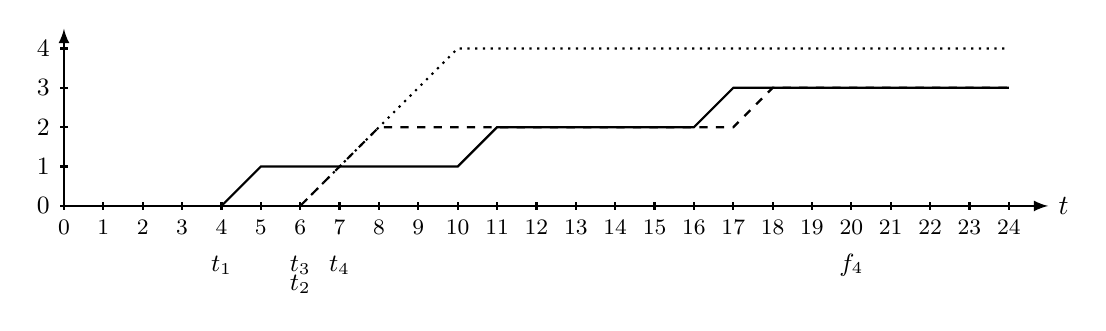
\begin{tikzpicture}[x=\ux,y=\uy, font=\sffamily,thick]  
		\tikzset{
			task/.style={fill=#1,  rectangle, text height=.3cm},
			task1a/.style={task=green!30},
			task1b/.style={task=green},
			task2a/.style={task=orange!30},
			task2b/.style={task=orange, minimum width=1mm},
			task3a/.style={task=pink, minimum width=1mm},
			task3b/.style={task=pink!80, minimum width=1mm},
			task4a/.style={task=cyan, minimum width=1mm},
			task4b/.style={task=cyan!50},
			task5/.style={task=blue},
			task6/.style={task=purple},
			task7/.style={minimum height=\ux,draw},
			task8/.style={minimum height=\ux,draw,thick},
			task9/.style={task=gray,minimum height=0.7cm,draw},
		}
		\tikzstyle{jobs}=[ fill=black!50];
		
		\draw[->] (0,0) -- coordinate (xaxis) (25,0) node[anchor=west] {$t$};
		\foreach \x in {0,...,24}{
			\draw[-](\x,0.1) -- (\x,-0.1)
			node[below] {\footnotesize $\x$};
			
		}
		\draw[->] (0,0) node[anchor=east] {}-- coordinate (xaxis) (0,4.5);
		\foreach \y in {0,...,4}{
			\draw[-](0.1, \y) -- (-0.1, \y)
			node[left] {\small $\y$};
			
		}

                \draw (20, -1.5) node {\small $f_4$};
                \draw (7, -1.5) node {\small $t_4$};
                \draw (6, -1.5) node {\small $t_3$};
                \draw (6, -2) node {\small $t_2$};
                \draw (4, -1.5) node {\small $t_1$};

                \draw[-,thick] (4,0) -- (5, 1) -- (10, 1) -- (11, 2) -- (16, 2)
                -- (17, 3) -- (22, 3) -- (23, 3) -- (24, 3);
                \draw[-,dashed] (6,0) -- (7, 1) -- (8, 2) -- (17, 2) -- (18, 3)
                -- (24, 3);
                \draw[-,dotted] (6,0) -- (10, 4) -- (24, 4);
		\end{tikzpicture}    
  \caption{The workload function for the three higher-priority tasks in Figure~\ref{fig:example-step2}. Solid line: $W_1^1(t-t_1)$, Dashed line: $W_2^0(t-t_2)$, Dotted line: $W_3^1(t-t_3)$, where the functions are $0$ if $t-t_j < 0$ for $j=1,2,3$.}
  \label{fig:example-step2}
\end{figure}

{\bf Step 3: Creating Safe Response-Time Analysis}


\begin{figure*}[t]
  \centering

		\def\ux{0.25cm}\def\uy{0.5cm} 
		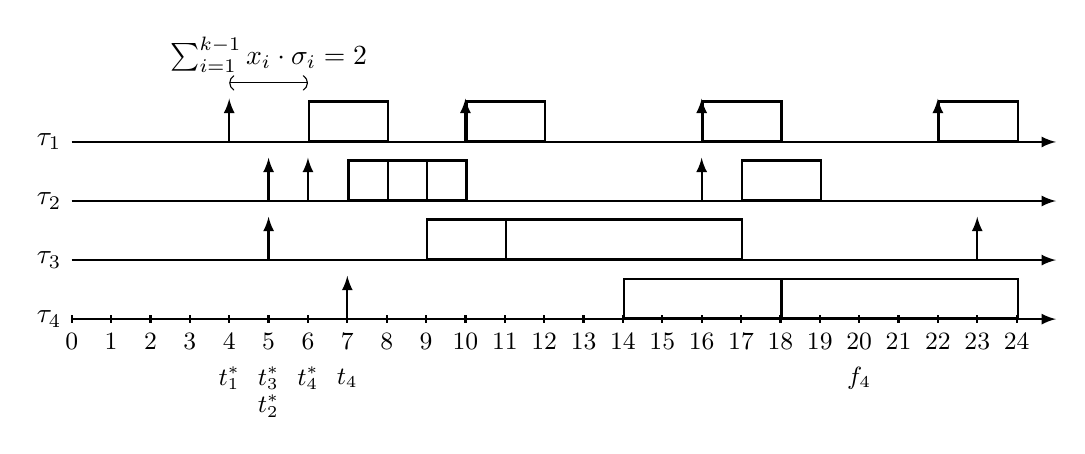
\begin{tikzpicture}[y=\uy, font=\sffamily,thick]  
		\tikzset{
			task/.style={fill=#1,  rectangle, text height=.3cm},
			task1a/.style={task=green!30},
			task1b/.style={task=green},
			task2a/.style={task=orange!30},
			task2b/.style={task=orange, minimum width=1mm},
			task3a/.style={task=pink, minimum width=1mm},
			task3b/.style={task=pink!80, minimum width=1mm},
			task4a/.style={task=cyan, minimum width=1mm},
			task4b/.style={task=cyan!50},
			task5/.style={task=blue},
			task6/.style={task=purple},
			task7/.style={minimum height=\ux,draw},
			task8/.style={minimum height=\ux,draw,thick},
			task9/.style={task=gray,minimum height=0.7cm,draw},
		}
		\tikzstyle{jobs}=[ fill=black!50];

		\begin{scope}[shift={(0,0)}]
		
		\draw[<-](2,1.1) -- (2,0);
		\draw[<-](5,1.1) -- (5,0);
		\draw[<-](8,1.1) -- (8,0);
		\draw[<-](11,1.1) -- (11,0);
		
		
		\draw[->] (0,0) node[anchor=east] {$\tau_1$}-- coordinate (xaxis) (12.5,0);

		
		\node[task7, minimum width=2*\ux,
		anchor=south west]at (3, 0){};
		\node[task7, minimum width=2*\ux,
		anchor=south west]at (5, 0){};
		\node[task7, minimum width=2*\ux,
		anchor=south west]at (8, 0){};
		\node[task7, minimum width=2*\ux,
		anchor=south west]at (11, 0){};
		\draw[(-), thin] (2, 1.5) -- (3, 1.5);
		\node[anchor=south] at (2.5, 1.5) {$\sum_{i=1}^{k-1} x_i \cdot \sigma_i=2$};

		\end{scope}
		
		
		\begin{scope}[shift={(0,-1.5)}]
		%%timeline
		
		
		\draw[<-](2.5,1.1) -- (2.5,0);
		\draw[<-](3,1.1) -- (3,0);
		\draw[<-](8,1.1) -- (8,0);
		
		
		\node[task7, minimum width=2*\ux,
		anchor=south west] at (3.5, 0){};
		\node[task7, minimum width=2*\ux,
		anchor=south west] at (4, 0){};
		\node[task7, minimum width=2*\ux,
		anchor=south west] at (8.5, 0){};

		\draw[->] (0,0)node[anchor=east] {$\tau_2$} -- coordinate (xaxis) (12.5,0);
		
		
		\end{scope}

		\begin{scope}[shift={(0,-3)}]
		%%timeline
		
		\draw[<-](2.5,1.1) -- (2.5,0);
		\draw[<-](11.5,1.1) -- (11.5,0);
		

		\draw[->] (0,0)node[anchor=east] {$\tau_3$} -- coordinate (xaxis) (12.5,0);
		
		\node[task7, minimum width=2*\ux,
		anchor=south west]  at ( 4.5, 0){};
		\node[task7, minimum width=6*\ux,
		anchor=south west]  at ( 5.5, 0){};
		
		\end{scope}

		\begin{scope}[shift={(0,-4.5)}]
		\draw[->] (0,0) node[anchor=east] {$\tau_4$}-- coordinate (xaxis) (12.5,0);
		\draw[<-](3.5,1.1) -- (3.5,0)node[anchor=north] {$$};
				\node[task7, minimum width=4*\ux,anchor=south west]at (7, 0){};
		\node[task7, minimum width=6*\ux,anchor=south west]at (9, 0){};
		
		\foreach \x in {0,...,24}{
			\draw[-](.5*\x,0.1) -- (.5*\x,-0.1)
			node[below] {\small $\x$};
			
		}

                \draw (10, -1.5) node {\small $f_4$};
                \draw (3, -1.5) node {\small $t_4^*$};
                \draw (3.5, -1.5) node {\small $t_4$};
                \draw (2.5, -1.5) node {\small $t_3^*$};
                \draw (2.5, -2.2) node {\small $t_2^*$};
                \draw (2, -1.5) node {\small $t_1^*$};
		\end{scope}
		
		\end{tikzpicture}  

\caption{An illustrative example of Step 3 in the proof of Theorem~\ref{theorem:general-framework} based on an \emph{imaginary} schedule.}
\label{fig:example-proof-final}  
\end{figure*}

This step constructs a safe response-time analysis based on the
conditions in Eqs.~(\ref{eq:exec_plus_idle-2}) and
(\ref{eq:exec_plus_idle-3}). We will construct another release pattern
which moves $t_i$ to $t_i^*$ for $i=2,3,\ldots,k$ such that $t_i^*
\leq t_i$ and the corresponding conditions in Eqs.~(\ref{eq:exec_plus_idle-2}) and
(\ref{eq:exec_plus_idle-3}) will become worse when we use $t_i^*$. We start
the procedure as follows:
\begin{itemize}
\item Initial Step: Let $t_1^*$ be $t_1$.
\item Iterative steps ($i=2,3,\ldots,k$): Let $t_i^*$ be $t_{i-1}^*+x_{i-1}\cdot\sigma_{i-1}$.
\end{itemize}
This results in $t_i^* \leq t_i$ for $i=2,3,\ldots,k$. Moreover, by
definition, $t_j^*$ is $t_1^* + \sum_{i=1}^{j-1} x_i\cdot\sigma_i$ for
$j=2,3,\ldots,k$.
For any task $\tau_j$ in ${\bf T}_1$,  $\forall \Delta \geq 0$, since $t_j \geq t_j^*$, we have
\begin{equation}
  \label{eq:execution-case1-shifted}
  W_j^1(\Delta)  \leq W_j^1(\Delta + (t_j-t_j^*)).
\end{equation}
For any task $\tau_j$ in ${\bf T}_0$,  $\forall \Delta \geq 0$, since $t_j \geq t_j^*$, we have
\begin{equation}
  \label{eq:execution-case2-shifted}
  W_j^0(\Delta)  \leq W_j^0(\Delta + (t_j-t_j^*)).
\end{equation}

Therefore, for any $j=1,2,\ldots,k-1$, the contribution $W_j^1(t-t_j)
\leq W_j^1(t-t_j^*)$ and $W_j^0(t-t_j) \leq W_j^0(t-t_j^*)$ for any $t
\geq t_j$. Putting these into 
Eqs.~(\ref{eq:exec_plus_idle-2}) $\forall t \mid t_k^* \leq t < t_k$ leads to
{\small \begin{align}
&\sum_{j=1}^{k-1} x_j\cdot (W_j^1(t-t_j^*)+\sigma_j) + (1-x_j)\cdot W_j^0(t-t_j^*) \geq t-t_1,\nonumber\\
\Rightarrow& \sum_{j=1}^{k-1} x_j\cdot W_j^1(t-t_j^*) + (1-x_j)\cdot W_j^0(t-t_j^*) \geq t-t_k^*.
\label{eq:exec_plus_idle-4}
\end{align}}
Similarly, putting these into 
Eqs.~(\ref{eq:exec_plus_idle-3}) $\forall t \mid t_k \leq t < f_k$ leads to 
\begin{equation}
\label{eq:exec_plus_idle-5}
C_k'+\sum_{j=1}^{k-1} x_j\cdot W_j^1(t-t_j^*) + (1-x_j)\cdot W_j^0(t-t_j^*) > t-t_k^*.
\end{equation}
 By the assumption that $C_k' \geq C_k > 0$, we can unify the above inequalities in Eq.~(\ref{eq:exec_plus_idle-4}) and Eq.~(\ref{eq:exec_plus_idle-5}) as follows:
$\forall t \mid t_k^* \leq t < f_k$
\begin{equation}
\label{eq:exec_plus_idle-almost-final} 
C_k'+\sum_{j=1}^{k-1} x_j\cdot W_j^1(t-t_j^*) + (1-x_j)\cdot W_j^0(t-t_j^*) > t-t_k^*.
\end{equation}



By definition, $\forall t \mid t_k^* \leq t < f_k$, we have
$t-t_j^* = t - t_k^* + \sum_{\ell=j}^{k-1} x_\ell\sigma_\ell$ for every
$j=1,2,\ldots,k-1$. Therefore, we know that
 $W_j^1(t-t_j^*) \leq
\ceiling{\frac{t-t_k^* +\sum_{\ell=j}^{k-1} x_\ell\sigma_\ell}{T_j}}C_j$ for task $\tau_j$ in ${\bf T}_1$. Moreover, 
$\forall t
\mid t_k^* \leq t < f_k$, we have $W_j^0(t-t_j^*) \leq
\ceiling{\frac{t-t_k^*+\sum_{\ell=j}^{k-1} x_\ell\sigma_\ell + (1-x_j)(D_j-C_j)}{T_j}}C_j$
for task $\tau_j$ in ${\bf T}_0$. Therefore, we can conclude that 
$\forall t \mid t_k^* \leq t < f_k$
\begin{equation}
C_k'+\sum_{j=1}^{k-1} \ceiling{\frac{t-t_k^*+X_j+(1-x_j)(D_j-C_j)}{T_j}} C_j > t-t_k^*,
\end{equation}
where $X_j$ is $\sum_{\ell=j}^{k-1} x_\ell\sigma_\ell$. We replace $t-t_k^*$ with $\theta$. 
The above inequation implies that the minimum $\theta$ with $\theta > 0$ such that
$C_k'+\sum_{j=1}^{k-1} \ceiling{\frac{\theta+X_j+(1-x_j)(D_j-C_j)}{T_j}} C_j = \theta$
 is larger than or equal to $f_k-t_k^* \geq f_k-t_k$. 

However, the above condition requires the knowledge of $\sigma_i$. It is straightforward to see that $\sum_{j=1}^{k-1} \ceiling{\frac{\theta+X_j+(1-x_j)(D_j-C_j)}{T_j}} C_j$ reaches the worst case if $X_j$ is the largest. Since $X_j$ is upper bounded by $Q_j^{\vec{x}}$ defined in Theorem~\ref{theorem:general-framework}, we reach the conclusion.

\noindent\underline{An example of the procedures in Step 3:} This can
be demonstrated in Figure~\ref{fig:example-proof-final} based on the
previous example in
Figure~\ref{fig:example}. Figure~\ref{fig:example-proof-final}
provides the imaginary workload and an imaginary execution plan based
on the test behind the condition in
Eq.~\eqref{eq:exec_plus_idle-almost-final}. \emph{Note that this is
  not an actual schedule since task $\tau_2$ is artificially alerted
  to release two jobs within a short time interval. This is only for
  illustrative purposes.}
For such a case, $t_1^*=4,
t_2^*=5, t_3^*=5$, and $t_4^*=6$. The two idle time units are used
between time $4$ and time $6$. The accumulated workload is then
started to be executed at time $6$ and the processor does not
idle after time $6$. Over here, we see that two jobs of task $\tau_2$ are executed
back to back from time 7 to time 9. As
shown in the imaginary schedule in
Figure~\ref{fig:example-proof-final}, the processor is busy executing
the workload from time $6$ to time $21$, which is more pessimistic
than the actual in Figure~\ref{fig:example}. The conclusion we have in the final statement of the theorem is that $20-7=f_k-r_k \leq 21-6$.
\end{appProof}


\begin{Lemma}
\label{lemma:Wj0-dominate}
$\forall \Delta \geq 0$ and $\forall C_j\geq c_j^* \geq 0$,
\[
\widehat{W}_j^0(\Delta, C_j)  \geq \widehat{W}_j^0(\Delta, c_j^*),
\]
where $\widehat{W}_j^0(\Delta, 0)$ is defined in Eq.~(\ref{eq:execution-case2-precise0}) and
 $\widehat{W}_j^0(\Delta, c_j^*)$ is defined in Eq.~(\ref{eq:execution-case2-precise}) if $c_j^* > 0$.
\end{Lemma}
\begin{proof}
  The proof is based on simple observations of the workload function. 
  We first prove that $\widehat{W}_j^0(\Delta, C_j) \geq
  W_j^1(\Delta)$ defined in Eq.~\eqref{eq:execution-case2-precise0}.  By the definition of $\rho_j=T_j-D_j+C_j$ when $c_j^*$ is $C_j$ and the
  assumption $C_j \leq D_j \leq T_j$, we have $0 \leq \rho_j \leq
  T_j$. Therefore, for $\Delta \geq T_j$, we have $W_j^1(\Delta) = C_j
  + W_j^1(\Delta-T_j) \leq C_j + W_j^1(\Delta - \rho_j) \leq
  \widehat{W}_j^0(\Delta, C_j)$. For $0 \leq \Delta < T_j$, it is also
  obvious that $\widehat{W}_j^0(\Delta, C_j) \geq \min\{\Delta, C_j\}
  = W_j^1(\Delta)$.

  We then prove that $\widehat{W}_j^0(\Delta, C_j) \geq
  \widehat{W}_j^0(\Delta, c_j^*)$ for any $0 < c_j^* \leq C_j$ based on the definition in Eq.~\eqref{eq:execution-case2-precise}. Figure~\ref{fig:example-lemma-workload} provides an illustrative example for $\widehat{W}_j^0(\Delta, c_j^*)$. We consider three subcases:
  \begin{compactitem}
  \item For $0 \leq \Delta \leq C_j$, it is obvious that
    $\widehat{W}_j^0(\Delta, C_j) \geq \widehat{W}_j^0(\Delta,
    c_j^*)$.
  \item For $C_j < \Delta \leq T_j-D_j+C_j$, we have
    $\widehat{W}_j^0(\Delta, C_j) = C_j$, and it is obvious that
    $\widehat{W}_j^0(\Delta, c_j^*) = c_j^* + \max\{0,
    \Delta-(T_j-D_j+c_j^*)\} \leq c_j^* + C_j - c_j^* = C_j$.

  \item For $T_j-D_j+C_j < \Delta$, we have $\widehat{W}_j^0(\Delta,
    C_j) = C_j + W_j^1(\Delta - (T_j-D_j+C_j))$.  Moreover, by
    definition, we also know $\widehat{W}_j^0(\Delta, c_j^*) \leq
    \delta+\widehat{W}_j^0(\Delta-\delta, c_j^*)$ for any $\delta$ with $0 < \delta \leq
    \Delta$. Therefore, for such a case, we can conclude
    $\widehat{W}_j^0(\Delta, c_j^*) = c_j^* + W_j^1(\Delta -
    (T_j-D_j+c_j^*)) \leq C_j + W_j^1(\Delta - (T_j-D_j+C_j))$ by
    setting $\delta$ to $C_j - c_j^*$ with the previous inequality.
  \end{compactitem}
\end{proof}


\begin{figure}[t]
  \centering

		\def\ux{0.32cm}\def\uy{0.3cm} 
		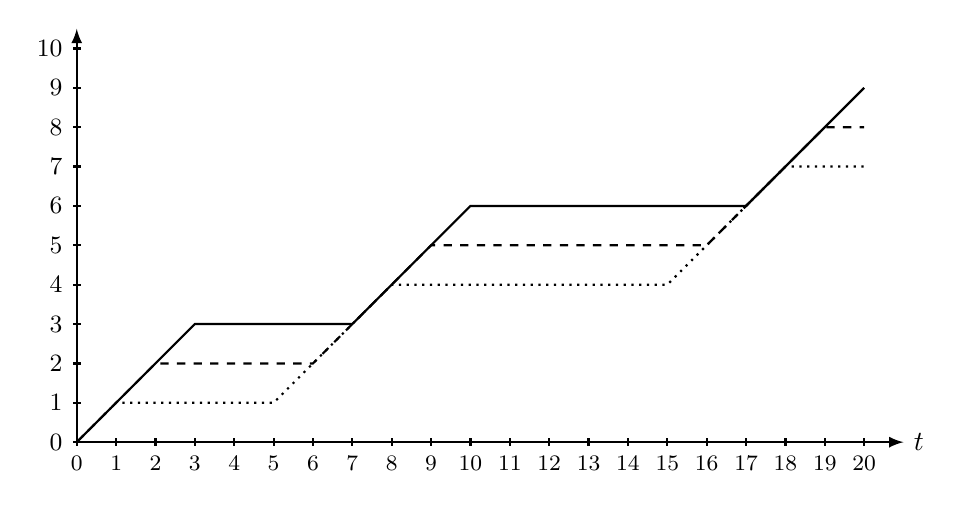
\begin{tikzpicture}[x=\ux,y=\uy, font=\sffamily,thick]  
		\draw[->] (0,0) -- coordinate (xaxis) (21,0) node[anchor=west] {$t$};
		\foreach \x in {0,...,20}{
			\draw[-](\x,0.1) -- (\x,-0.1)
			node[below] {\footnotesize $\x$};
			
		}
		\draw[->] (0,0) node[anchor=east] {}-- coordinate (xaxis) (0,10.5);
		\foreach \y in {0,...,10}{
			\draw[-](0.1, \y) -- (-0.1, \y)
			node[left] {\small $\y$};
			
		}

                \draw[-,thick] (0, 0) -- (3, 3) -- (7, 3) -- (10, 6) -- (17, 6) -- (20, 9);
                \draw[-,dashed] (0 ,0) -- (2,2) -- (6, 2) -- (9, 5) -- (16, 5) -- (19, 8) -- (20, 8);
                \draw[-,dotted] (0, 0) -- (1, 1) -- (5, 1) -- (8, 4) -- (15, 4) -- (18, 7) -- (20, 7);
		\end{tikzpicture}    
  \caption{The workload function $\widehat{W}_j^0(\Delta, c_j^*)$ when $T_j=10$, $C_j=3$, and $D_j=6$. Solid line: $c_j^*$ is $3$, Dashed line: $c_j^*$ is $2$, Dotted line: $c_j^*$ is $1$.}
  \label{fig:example-lemma-workload}
\end{figure}

\section{Proof of Correctness}  
\label{sec:proof-th1}
\ifpaper
\newtheorem{property}{Property}
\newtheorem{lemma}{Lemma}
\newtheorem{corollary}{Corollary}
\fi
\section{Proof of Liu's Analysis}  

This section provides the proof to support the correctness of the test in Eq. \eqref{eq:TDA-suspension}. First, it should be easy to see that we can convert the suspension time of task $\tau_k$ into computation. This has been proven in many previous works, e.g., Lemma~3 in \cite{Liu_2014} and Theorem~2 in \cite{ecrts15nelissen}. Yet, it remains to formally prove that the additional interference due to the self-suspension of a higher-priority task $\tau_i$ is upper-bounded by $b_i=min(C_i, S_i)$. The interference to be at most $C_i$ has been provided in the literature as well, e.g., \cite{Rajkumar_1990,Liu_2014}. However, the argument about blocking task $\tau_k$ due to a higher-priority task $\tau_i$ by at most $S_i$ amount of time is not straightforward. 

From the above discussions, we can greedily convert the suspension time of task $\tau_k$ to its computation time. For the sake of notational brevity, let $C_k'$ be $C_k + S_k$. We call this converted version of task $\tau_k$ as task $\tau_k'$. Our analysis is also based on very simple properties and lemmas enunciated as follows:

\begin{property}
\label{prop:lower-priority}
In a preemptive fixed-priority schedule, the lower-priority jobs do not impact the schedule of the higher-priority jobs.
\end{property}

%\begin{lemma}
%\label{lemma:remove-lower-priority}
%In a preemptive fixed-priority schedule, removing a lower-priority job arrived at time $t$ does not affect the schedule of the higher-priority jobs after time $t$.
%\end{lemma}
%\begin{proof}
%This is a direct consequence of Property~\ref{prop:lower-priority}.
%\end{proof}

\begin{lemma}
\label{lemma:remove-same-task}
In a preemptive fixed-priority schedule, if the worst-case response time of task $\tau_i$ is no more than its period $T_i$, removing a job of task $\tau_i$ does not affect the schedule of any other job of task $\tau_i$.
\end{lemma}
\begin{proof}
Since the worst-case response time of task $\tau_i$ is no more than its period, any job $\tau_{i,j}$ of task $\tau_i$ completes its execution before the release of the next job $\tau_{i,j+1}$. Hence, the execution of $\tau_{i,j}$ does not interfere with the execution of any other job of $\tau_i$, which then depends only on the schedule of the higher priority jobs. Furthermore, as stated in Property~\ref{prop:lower-priority}, the removal of $\tau_{i,j}$ has no impact on the higher-priority jobs, thereby implying that the other jobs of task $\tau_i$ are not affected by the removal of $\tau_{i,j}$.
\end{proof}

We can prove the correctness of Eq. \eqref{eq:TDA-suspension} by using a similar proof of the critical instant theorem of the ordinary sporadic task system.
Let $R_k'$ be the minimum $t > 0$ such that  $C'_k + B_k + \sum_{i=1}^{k-1}\ceiling{\frac{t}{T_i}} C_i = t$, i.e., Eq. \eqref{eq:TDA-suspension} holds. The following lemma shows that $R_k'$ is a safe upper bound if the worst-case response time of task $\tau_k'$ is no more than $T_k$.

\begin{theorem}
\label{theorem:critical}
 $R_k'$ is a safe upper bound on the worst-case response time of task $\tau_k'$ if the worst-case response time of $\tau_k'$ is not larger than $T_k$.
\end{theorem}
\begin{proof}
Let us consider the task set $\tau'$ composed of $\left\{\tau_1, \tau_2, \ldots, \tau_{k-1}, \tau_k', \tau_{k+1}, \ldots \right\}$ and let $S$ be a schedule of $\tau'$ that generates the worst-case response time of $\tau_k'$. Suppose that the job $J_{k}$ of task $\tau_k'$ with the largest response time in $S$ arrives at time $r_k$ and finishes at time $\rho$. We know by Property~\ref{prop:lower-priority} that the lower priority tasks $\tau_{k+1}, \tau_{k+2}, \ldots$ do not impact the response time of $J_{k}$. Moreover, since we assume that the worst-case response time of task $\tau_k'$ is no more than $T_k$, Lemma~\ref{lemma:remove-same-task} proves that removing all the jobs of task $\tau_k'$ but $J_{k}$ has no impact on the schedule of $J_{k}$ arrived at time $r_k$. Therefore, let $S^{red}$ be a schedule identical to $S$ but removing all the jobs released by the lower priority tasks $\tau_{k+1}, \tau_{k+2}, \ldots$ as well as all the jobs released by $\tau_k'$ at the exception of $J_{k}$. The response time of $J_{k}$ in $S^{red}$ is identical to the response time of $J_{k}$ in $S$.


Therefore, for the rest of the proof, we only have to consider this \emph{reduced} schedule $S^{red}$. Note that by construction of $S^{red}$, the processor is busy only when executing higher-priority tasks than $\tau'_k$ or the job of task $\tau_k'$ released at time $r_k$ and completing at time $\rho$. In $S^{red}$, let $t_{k}$ be the latest moment before $r_k$ such that the processor does not execute any job. That is, from $t_k$ to $r_k$, the processor executes tasks with higher priorities than $\tau_k'$. Apparently, one can change the release time of the unique job of task $\tau_k'$ in $S^{red}$ to time $t_k$, and hence increase the response time of the job to $\rho-t_k \geq \rho-r_k$. It however contradicts our assumption that the response time of $J_{k}$ is the worst-case response time of $\tau_k'$. Consequently, $t_k$ is equal to the release $r_k$ of $J_{k}$ in $S^{red}$ and the processor is idle before $t_k$.

Up to here, the proof is basically similar to the proof of the critical instant theorem of the usual sporadic sequential real-time task model. However, for self-suspending tasks, one needs to consider that a job of a higher priority task $\tau_i$ can suspend itself before $t_k$ and resume its execution after $t_k$. Such jobs are usually referred to as \emph{carry-in} jobs. %Fortunately, each higher-priority task has only one carry-in job due to the assumption that the higher-priority tasks are assumed to finish before their periods. However, analyzing the accurate workload of such jobs due to self-suspension is non-trivial. 
%One can conclude that each job of task $\tau_i$ has execution time up to $C_i$. This is fine with $S_i \geq C_i$. If $S_i < C_i$, we explain how to further extend the analysis window further iteratively. For the simplicity of presentation, let $J_i$ be the carry-in job of task $\tau_i$ at time $t_k$.

The proof is built upon the two following steps:
\begin{enumerate}
\item First, we extend the window of interest from $[t_k, \rho)$ to a larger time window $[t_1, \rho)$ by iteratively inspecting the schedule of the higher priority tasks in $S^{red}$, starting with $\tau_{k-1}$ until the highest priority task $\tau_1$. At each iteration, the window of interest is extended from $[t_{j+1}, \rho)$ to $[t_{j}, \rho)$ with $t_j \leq t_{j+1}$ ($1 \leq j < k$). Once $t_j$ has been identified, all the jobs of task $\tau_j$ released before $t_j$ are removed and, if needed, replaced by an artificial job to consider the residual workload of task $\tau_j$ at time $t_j$ impacting the response time of $J_{k}$. 
\item Second, the final reduced schedule is analyzed in the time window $[t_1, \rho)$ to characterize the response time of $J_{k}$ and hence the worst-case response time of $\tau_k$.
\end{enumerate}

{\bf Step 1: Extending the Window of Interest} 

Let $S^k$ be a schedule exactly identical to $S^{red}$. During this step, we iteratively build an artificial schedule $S^j$ from $S^{j+1}$ (with $1 \leq j < k$) so that the response time of $J_{k}$ can only increase. As already discussed above, let $t_k$ be equal to $r_k$ in $S^k$. At each iteration, we define $t_j$ for task $\tau_j$ in the schedule $S^{j+1}$ (with $j=k-1, k-2, \ldots, 1$) and build $S^j$ by removing all the jobs released by $\tau_j$ before $t_j$.


Let $r_j$ be the arrival time of the last job released by $\tau_j$ before $t_{j+1}$ in $S^{j+1}$ and let $J_{j}$ denote that job. %There are a two possible cases:
%\begin{itemize}
%\item $J_{j}$ completed its execution no later than $t_{j+1}$. Then, we simply set $t_j$ to $t_{j+1}$ and generate $S^j$ by removing all the jobs of task $\tau_j$ arrived before $t_{j+1}$ in the schedule $S^{j+1}$. By Lemma~\ref{lemma:remove-same-task} and Property \ref{prop:lower-priority}, removing all the jobs of task $\tau_j$ arrived before $t_{j+1}$ has no impact on the schedule of the higher-priority jobs (jobs released by $\tau_1, \ldots, \tau_{j-1}$) and the jobs of $\tau_j$ released after $t_{j+1}$. Moreover, because no task with a priority lower than $\tau_j$ executes jobs before $t_{j+1}$ in $S^{j+1}$, removing the jobs released by $\tau_j$ before $t_{j+1}$ does not impact the schedule of the jobs of $\tau_{j+1}, \ldots, \tau_{k}$. The response time of $J_{k}$ in $S^j$ thus remains unchanged in comparison to its response time in $S^{j+1}$. 
%\item $J_{j}$ did not complete its execution before $t_{j+1}$.
Removing all the jobs of task $\tau_j$ arrived before $r_j$ has no impact on the schedule of any other job released by $\tau_j$ (Lemma~\ref{lemma:remove-same-task}) or any higher priority job released by $\tau_1, \ldots, \tau_{j-1}$ (Property \ref{prop:lower-priority}). Moreover, because by construction of $S^{j+1}$, no task with a priority lower than $\tau_j$ executes jobs before $t_{j+1}$ in $S^{j+1}$, removing the jobs released by $\tau_j$ before $t_{j+1}$ does not impact the schedule of the jobs of $\tau_{j+1}, \ldots, \tau_{k}$. Therefore, we can safely remove all the jobs of task $\tau_j$ arrived before $r_j$ without impacting the response time of $J_{k}$. Two cases must then be considered:
\begin{enumerate}[(a)]
\item $\tau_j \in {\bf T}_1$, i.e., $S_j < C_j$. For such a case, $t_{j}$ is set to $r_j$ and hence $S^j$ is built from $S^{j+1}$ by removing all the jobs released by $\tau_j$ before $r_j$. Note that because by construction of $S^{j+1}$ and hence $S^j$ there is no job with priority lower than $\tau_j$ available to be executed before $t_{j+1}$, the maximum amount of time during which the processor remains idle within $[t_j, t_{j+1})$ is at most $S_j$ time units.
\item $\tau_j \in {\bf T}_2$, i.e., $S_j \geq C_j$. For such a case, we set $t_{j}$ to $t_{j+1}$. Let $c_j(t_j)$ be the remaining execution time for the job of task $\tau_j$ at time $t_j$. We know that $c_j(t_j)$ is at most $C_j$. Since by construction of $S^j$, all the jobs of $\tau_j$ released before $t_j$ are removed, the job of task $\tau_j$ arrived at time $r_j$ ($< t_j$) is replaced by a new job released at time $t_j$ with execution time $c_j(t_j)$ and the same priority than $\tau_j$. Clearly, this has no impact on the execution of any job executed after $t_j$ and thus on the response time of $J_k$. The remaining execution time $c_j(t_j)$ of $\tau_j$ at time $t_j$ is called the \emph{residual workload} of task $\tau_j$ in the rest of the proof.
\end{enumerate}
%\end{itemize}
 
%The above construction of $t_{k-1}, t_{k-2}, \ldots, t_1$ is well-defined. After each iteration to set $t_j$, we can reduce the schedule by removing some jobs without affecting the schedule of the carry-in $J_j$. (Note that $J_j$ is defined as the carry-in job of task $\tau_j$ at time $t_k$.) Therefore, the reduced schedule after the above procedure does not change the execution of $J_j$ after time $t_j$ if $\tau_j$ is in ${\bf T}_1$. For a task $\tau_j$ in ${\bf T}_2$, its corresponding carry-in job $J_j$ may be changed, but its execution after $t_j$ remains identical as in the original schedule. 
%Therefore, the resulting schedule above does not change any execution behavior of the (at most) $k-1$ carry-in jobs at time $t_k$.

{\bf Step 2: Analyze the Final Reduced Schedule in $[t_1, \rho)$:}


We now analyze the properties of the final schedule $S^1$ in which all the unnecessary jobs have been removed.   

From case (b) of Step 1, the total residual workload that must be considered in $S^1$ is upper bounded by $\sum_{\tau_i \in {\bf T}_2} C_i$.
%Consequently, for any time $t$ such that $t_1 < t \leq \rho$, the total amount of idle time and residual workload within $[t_1, t)$ is upper bounded by $\sum_{\tau_i \in {\bf T}_1} S_i + \sum_{\tau_i \in {\bf T}_2} C_i = \sum_{i=1}^{j} b_i$. 
Therefore, considering the fact that no job of $\tau_j$ is released before $t_j$ in $S^1$ ($j=1,2,\ldots,k-1$), the workload released by the tasks within any time interval $[t_1, t)$ such that $t_1 < t \leq \rho$ is upper bounded by 
\begin{align*}
\sum_{i=1}^k \left( c_j(t_j) + \max\{0, \ceiling{\frac{t- t_i}{T_i} } C_i \} \right) & \leq \sum_{\tau_i \in {\bf T}_2} C_i + \sum_{i=1}^k \max\{0, \ceiling{\frac{t- t_i}{T_i} } C_i \}
\end{align*}
%\[
%\forall t_j \leq t < t_{j+1},\qquad  \sum_{i=1}^{j} b_i + \sum_{i=1}^j %\ceiling{\frac{t- t_i}{T_i} } C_i >  t-t_1.
%\]
%By further considering the time interval from $t_k$ to $\rho$, we have
%\[
%\forall t_k \leq t < \rho,\qquad  C_k'+\sum_{i=1}^{k-1} b_i + \sum_{i=1}^{k-1} \ceiling{\frac{t- t_i}{T_i} } C_i > t-t_1.
%\]

Furthermore, from case (a) of Step 1, we know that the maximum amount of time during which the processor is idle in $S^1$ within any time interval $[t_1, t)$ such that $t_1 < t \leq t_k$, is upper bounded by $\sum_{\tau_i \in {\bf T}_1} S_i$. %We can simply consider such self-suspension time as \emph{virtual computation}.
Hence, adding that time to the maximum workload released by the tasks within any time interval $[t_1, t)$ such that $t_1 < t \leq t_k$, it holds that
\[
\forall t \mid t_1 \leq t < t_k,\qquad  \sum_{\tau_i \in {\bf T}_1} S_i + \sum_{\tau_i \in {\bf T}_2} C_i + \sum_{i=1}^{k} \max\{ 0, \ceiling{\frac{t- t_i}{T_i} } C_i\}  \geq t-t_1
\]
Considering that $C_k' > 0$ and that $\max\{ 0, \ceiling{\frac{t- t_k}{T_k} } C_k\} = 0$ for any $t$ smaller than $t_k$, we get that
\[
\forall t \mid t_1 \leq t < t_k,\qquad  \sum_{\tau_i \in {\bf T}_1} S_i + \sum_{\tau_i \in {\bf T}_2} C_i + C_k' + \sum_{i=1}^{k-1} \max\{ 0, \ceiling{\frac{t- t_i}{T_i} } C_i\}  > t-t_1
\]
and simplifying using the definition of $b_i$
\begin{equation}
\label{eq:eq1_in_proof}
\forall t \mid t_1 \leq t < t_k,\qquad  C_k'+\sum_{i=1}^{k-1} b_i + \sum_{i=1}^{k-1} \max\{ 0, \ceiling{\frac{t- t_i}{T_i} } C_i\} \geq t-t_1
\end{equation}

Additionally, because $J_k$, which is released at time $t_k$, does not complete its execution before $\rho$, it must hold that
\begin{equation}
\label{eq:eq1_in_proof}
\forall t \mid t_k \leq t < \rho,\qquad  C_k'+\sum_{i=1}^{k-1} b_i + \sum_{i=1}^{k-1} \max\{ 0, \ceiling{\frac{t- t_i}{T_i} } C_i\} > t-t_1.
\end{equation}

Since $t_i \geq t_1$ for $i=1,2,\ldots,k$, there is 
$$\ceiling{\frac{t- t_i}{T_i} } \leq \ceiling{\frac{t- t_1}{T_i} }$$ and without any loss of generality, by arbitrarily assuming $t_1 =0$, Inequation~\ref{eq:eq1_in_proof} becomes
\[
\forall t \mid 0 < t < \rho, \qquad C_k'+\sum_{i=1}^{k-1} b_i + \sum_{i=1}^{k-1} \ceiling{\frac{t}{T_i} } C_i > t.
\]
The above inequation implies that the minimum $t$ such that $C_k'+\sum_{i=1}^{k-1} b_i + \sum_{i=1}^{k-1} \ceiling{\frac{t}{T_i} } C_i \leq t$ is larger than or equal to $\rho$. And because by assumption the worst-case response time of $\tau_k'$ is equal to $\rho-t_k$ which is obviously smaller than or equal to $\rho$, it holds that $R_k'$ is a safe upper bound on the worst-case response time of $\tau_k'$.
\end{proof}

\begin{corollary}
\label{cor:critical}
 $R_k'$ is a safe upper bound on the worst-case response time of task $\tau_k'$ if $R_k'$ is not larger than $T_k$.
\end{corollary}
\begin{proof}
Directly follows from Theorem~\ref{theorem:critical}.
\end{proof}



\begin{corollary}
$R'_k$ is a safe upper bound on the worst-case response time of task $\tau_k$ if $R_k'$ is not larger than $T_k$. 
\end{corollary}
\begin{proof}
Since, as proven in \cite{Rajkumar_1990,Liu_2014}, the worst-case response time of $\tau_k'$ is always larger than or equal to the worst-case response time of $\tau_k$, this corollary directly follows from Corollary~\ref{cor:critical}. 
\end{proof}


  
To illustrate Step 1 in the above proof, we also provide one concrete example. Consider a task system with the following 4 tasks:
\begin{itemize}
\item $T_1 = 6, C_1 = 1, S_1 = 1$,
\item $T_2 = 10, C_2 = 1, S_2 = 6$,
\item $T_3 = 18, C_3 = 4, S_3 = 1$,
\item $T_4 = 20, C_4 = 5, S_4 = 0$.
\end{itemize}

Figure~\ref{fig:example} demonstrates a schedule for the jobs of the
above 4 tasks. We assume that the first job of task $\tau_1$ arrives
at time $4+\epsilon$ with a very small $\epsilon > 0$. The first job
of task $\tau_2$ suspends itself from time $0$ to time $5+\epsilon$,
and is blocked by task $\tau_1$ from time $5+\epsilon$ to time
$6+\epsilon$. After some very short computation with $\epsilon$ amount
of time, the first job of task $\tau_2$ suspends itself again from
time $6+2\epsilon$ to $7$.   In this schedule, $\rho$ is set to $20-\epsilon$.

We define $t_4$ as $7$. Then, we set $t_3$ to $6$. When considering
task $\tau_2$, since it belongs to ${\bf T}_2$, we greedily set $t_2$
to $t_3=6$ and the residual workload $C_2'$ is $1$. Then, $t_1$ is set
to $4+\epsilon$. In the above schedule, the idle time from
$4+\epsilon$ to $20-\epsilon$ is at most $2 = S_1+S_3$. We have to
further consider one job of task $\tau_2$ arrived before time $t_1$
with execution time $C_2$.
  
  
  

%%% Local Variables:
%%% mode: latex
%%% TeX-master: "authorea_build/authorea_paper.tex"
%%% End:


\chapter{Dominance over the State of the Art}
\label{sec:dominance}
\section{Dominance over the State of the Art}
\label{sec:dominance}

In this section, we prove that the schedulability test presented in Corollary~\ref{corollary:general-framework} dominates all the existing tests in the state-of-the-art, in the sense that if a task set is deemed schedulable by either of the tests presented in Section~\ref{sec:existing-analyses}, then it is also deemed schedulable by Corollary~\ref{corollary:general-framework}.

\begin{Lemma}
\label{lem:dominance_oblivious}
  The schedulability test of task $\tau_k$ provided by
  Eq.~\eqref{eq:TDA-suspension} dominates that of
  Eq.~\eqref{eq:TDA-SO}.
\end{Lemma}
\begin{proof}
For any $t > 0$, it is straightforward to see that
\begin{align*}
& C_k + S_k + \sum_{i=1}^{k-1}\ceiling{\frac{t}{T_i}} (C_i + S_i) \\
 \geq & C_k + S_k + \sum_{i=1}^{k-1} S_i + \sum_{i=1}^{k-1}\ceiling{\frac{t}{T_i}} C_i\\
 \geq & C_k + S_k + \sum_{i=1}^{k-1} \min(C_i, S_i) + \sum_{i=1}^{k-1}\ceiling{\frac{t}{T_i}} C_i
\end{align*}
and by using the definition of $B_k$ (i.e., in Section~\ref{sec:suspension-blocking}), we get
\begin{align*}
C_k + S_k + \sum_{i=1}^{k-1}\ceiling{\frac{t}{T_i}} (C_i + S_i) \geq C_k + B_k + \sum_{i=1}^{k-1}\ceiling{\frac{t}{T_i}} C_i
\end{align*}
Therefore, Eq.~\eqref{eq:TDA-suspension} will always have a solution which is smaller than or equal to the solution of Eq.~\eqref{eq:TDA-SO}. This proves the lemma.
\end{proof}

\begin{Lemma}
  \label{lem:dominance_jitter}
  The schedulability test presented in
  Corollary~\ref{corollary:general-framework} dominates the
  schedulability test provided by Eq.~\eqref{eq:TDA-jitter}.
\end{Lemma}
\begin{proof}
  Consider the case where $x_1=x_2=\cdots=x_{k-1}=0$. Eq.~\eqref{eq:TDA-suspension-tighter} becomes identical to Eq.~\eqref{eq:TDA-jitter} for this particular vector assignment. Therefore, if Eq.~\eqref{eq:TDA-jitter} deems a task set as being schedulable, so does Corollary~\ref{corollary:general-framework}. This proves the lemma. 
\end{proof}
  
\begin{Lemma}
  \label{lem:dominance_blocking}
  The schedulability test presented in
  Corollary~\ref{corollary:general-framework} dominates the
  schedulability test provided by Eq.~\eqref{eq:TDA-suspension}.
\end{Lemma}
\begin{proof}
  In this proof, we first transform the worst-case response time analysis presented in Corollary~\ref{corollary:general-framework} in a more pessimistic analysis. We then prove that this more pessimistic version of Corollary~\ref{corollary:general-framework} provides the same solution as Eq.~\eqref{eq:TDA-suspension}, which then proves the lemma. Due to space limitation, the proof is in Appendix\citetechreport{}.
\end{proof}

\begin{theorem}
  \label{theorem:dominance}
  The schedulability test presented in Corollary~\ref{corollary:general-framework} dominates the schedulability tests provided by Equations~\eqref{eq:TDA-SO}, \eqref{eq:TDA-jitter}, and~\eqref{eq:TDA-suspension}.
\end{theorem}
\begin{proof}
It is a direct application of Lemmas~\ref{lem:dominance_oblivious}, \ref{lem:dominance_jitter} and~\ref{lem:dominance_blocking}.
\end{proof}


As a corollary of this theorem, it directly follows that all the response time analyses discussed in Section~\ref{sec:existing-analyses} are in fact correct. This provides the first proof of correctness for Eq.~\eqref{eq:TDA-suspension}, which was initially presented in \cite{Liu:2000:RS:518501} but never proven correct.

\begin{theorem}
  \label{theorem:correctness_soa}
  The schedulability tests provided by Eqs~\eqref{eq:TDA-SO}, \eqref{eq:TDA-jitter}, and~\eqref{eq:TDA-suspension} are all correct.
\end{theorem}
\begin{proof}
It directly results from the two following facts,
\begin{compactitem}
\item[(i)] by Theorem~\ref{theorem:dominance}, the schedulability test presented in Corollary~\ref{corollary:general-framework} dominates the schedulability tests provided by Equations~\eqref{eq:TDA-SO}, \eqref{eq:TDA-jitter}, and~\eqref{eq:TDA-suspension};
\item [(ii)] as proven in Section~\ref{sec:proof-th1}, Corollary~\ref{corollary:general-framework} is correct.
\end{compactitem}
\end{proof}




%%% Local Variables:
%%% mode: latex
%%% TeX-master: "master.tex"
%%% End:


\chapter{Linear Approximation}
\label{sec:linear-approximation}
\section{Linear Approximation}
\label{sec:linear-approximation}

To test the schedulability of task $\tau_k$,
Corollary~\ref{corollary:general-framework} implies to test all the
possible vector assignments $\vec{x} = (x_1, x_2, \ldots, x_{k-1})$, in which there are $2^{k-1}$
different combinations. Therefore, the time complexity becomes
exponential if we consider all the vector assignments. Therefore, in this section, we provide a solution to reduce the time complexity associated to
Corollary~\ref{corollary:general-framework}. 

Hence, we explain how to use the linear approximation of the test in Eq.~(\ref{eq:TDA-suspension-tighter}) to help derive a good vector assignment. By the definition of $\ceiling{x}$, we have the following inequality:
{\small \begin{align}
&C_k'+ \sum_{i=1}^{k-1}\ceiling{\frac{t+\sum_{\ell=i}^{k-1}x_\ell S_\ell+(1-x_i)(D_i-C_i)}{T_i}} C_i \nonumber\\
\leq& C_k' +   \sum_{i=1}^{k-1} \left(\frac{t+\sum_{\ell=i}^{k-1}x_\ell S_\ell +(1-x_i)(D_i-C_i)}{T_i} +1\right) C_i \nonumber\\
=& C_k' + \sum_{i=1}^{k-1} \left(U_i\cdot t + C_i+U_i (1-x_i)(D_i-C_i) + U_i\sum_{\ell=i}^{k-1}x_\ell S_\ell \right)\nonumber\\
=& C_k' + \sum_{i=1}^{k-1}  \left(U_i\cdot t + C_i + U_i (1-x_i)(D_i-C_i) + x_i S_i\left(\sum_{\ell=1}^{i}U_\ell\right)\right)\label{eq:linear-approximation-upper-bound}
\end{align}}

By observing Eq.~(\ref{eq:linear-approximation-upper-bound}), the
contribution of $x_i$ can be individually determined as $U_i(D_i-C_i)$
when $x_i$ is $0$ or $S_i(\sum_{\ell=1}^{i}U_\ell)$ when $x_i$ is
$1$. Therefore, whether $x_i$ should be set to $0$ or $1$ can be
easily decided by individually comparing the two constants
$U_i(D_i-C_i)$ and $S_i(\sum_{\ell=1}^{i}U_\ell)$. We denote the
vector assignment obtained above by $\vec{x}^{linear}$. That is, for
each higher-priority task $\tau_i$,
\begin{itemize}
\item if $U_i(D_i-C_i) > S_i(\sum_{\ell=1}^{i}U_\ell)$, we greedily set $x_i^{linear}$ to $1$; 
\item otherwise, we greedily set $x_i^{linear}$ to $0$. 
\end{itemize}

For notational brevity, we denote the right-hand side of
Eq.~(\ref{eq:linear-approximation-upper-bound}) as $rbf_k(t, \vec{x})$
for any $t > 0$ and given $\vec{x}$.
\begin{theorem}
\label{theorem:linear-time-test}
  For any $t > 0$, the vector assignment $\vec{x}^{linear}$ minimizes
  $rbf_k(t, \vec{x})$ among all $2^{k-1}$ possible vector assignments
  for the $k-1$ higher-priority tasks. Task $\tau_k$ is schedulable
  under the fixed-priority scheduling if
  \begin{equation}
    \label{eq:linear-time-test}
    rbf_k(D_k, \vec{x}^{linear}) \leq D_k.
  \end{equation}
  Deriving $\vec{x}^{linear}$ requires $O(k)$ time complexity and
  testing Eq.~(\ref{eq:linear-approximation-upper-bound}) also
  requires only $O(k)$ time complexity.
\end{theorem}
\begin{proof}
  The correctness to test Eq.~\eqref{eq:linear-time-test} is due to
  the derivation in Eq.~\eqref{eq:linear-approximation-upper-bound}
  and Corollary~\ref{corollary:general-framework}. The other
  statements in this theorem are based on the above discussion in this
  section and simple observations.
\end{proof}


% \begin{Corollary}
%   \label{corollary:linear-time-overall-test}
%   Considering task $\tau_k$ from $\tau_1, \tau_2, \ldots, \tau_n$, the
%   time complexity to test the schedulability of all these $n$ tasks is
%   $O(n)$ by using the test in
%   Theorem~\ref{theorem:linear-time-test}. Therefore, the amortized
%   time complexity to test task $\tau_k$ by using the test in
%   Theorem~\ref{theorem:linear-time-test} is constant.
% \end{Corollary}
% \begin{proof}
  
% \end{proof}









\chapter{Experiments}
\label{sec:experiments}

\section{Experiments}
\label{sec:experiments}

In this section, we present experiments conducted on randomly generated task sets. Five schedulability tests for dynamic self-suspending tasks are compared, namely, the suspension oblivious approach (Section~\ref{sec:suspension-oblivious}), the modeling of suspension as a release jitter (Section~\ref{sec:jitter}), the analysis proposed by Jane W.S. Liu and proven correct in this paper, which models the suspension as blocking (Section~\ref{sec:suspension-blocking}), the generic framework of Corollary~\ref{corollary:general-framework} (called ECRTS 16 in the graph) and the test based on the linear approximation presented in Section~\ref{sec:linear-approximation}. Each point in the plots of Figure~\ref{fig:exp} represents the number of task sets that were deemed schedulable by the respective algorithm over $1000$ experiments.

The task sets were generated using the \texttt{randfixedsum} algorithm presented in \cite{Emberson-taskSetGeneration-2010}.


\begin{figure*}[t!]
  \centering
  \small
  \subfloat[$U=0.95$, $S_i \in (0.05, 0.50) \times C_i$]{\label{fig:plot1} \includegraphics[width=0.48\textwidth]{../figures/experiments/varyingn_smin=5_smax=50_U=0_95_T=100-10000_1000runs.pdf}} 
  \subfloat[$U=1$, $n=8$]{\label{fig:plot2} \includegraphics[width=0.48\textwidth]{../figures/experiments/varyingSmax_smin=5_U=1_n=8_T=100-10000_1000runs.pdf}}\\ 
  \subfloat[$U=1$, $n=8$, $S_i\in (0.05, 0.50) \times C_i$]{\label{fig:plot3} \includegraphics[width=0.48\textwidth]{../figures/experiments/varyingU_smin=5_smax=50_n=8_T=100-10000_1000runs.pdf}}
  \subfloat[$U=1$, $n=8$, $S_i\in (0.50, 0.90) \times C_i$]{\label{fig:plot4} \includegraphics[width=0.48\textwidth]{../figures/experiments/varyingU_smin=50_smax=90_n=8_T=100-10000_1000runs.pdf}} 
  \caption{Number of schedulable task sets over $1000$ randomly generated task sets.}
  \label{fig:exp}
\end{figure*}



\chapter{Conclusion}
\label{sec:conclusion}


In this paper, we studied the preemptive fixed-priority scheduling of
dynamic self-suspending tasks running on a uniprocessor platform. This
paper presents a unifying response time analysis framework in
Theorems~\ref{theorem:general-framework}~\ref{theorem:general-framework-not-feasible} and
Corollary~\ref{corollary:general-framework}. We show that this result
analytically dominates all the existing analyses presented in
Section~\ref{sec:existing-analyses}, and, by doing such, we also implicitly
proved the correctness of all these analyses. Although
Corollary~\ref{corollary:general-framework} requires exponential time
complexity, we show that a simpler algorithm presented in Section~\ref{sec:linear-approximation} can help accelerate the analysis while outputting good results.

%In fact, the response time analysis and the schedulability tests in
%Section~\ref{sec:existing-analyses} and
%Theorem~\ref{theorem:general-framework} can be further approximated to
%polynomial-time complexity. For example, by over-approximating the
%jitter used in Section~\ref{sec:jitter}, Liu and Chen
%in \cite{LiuChen:rtss2014} provided a utilization-based schedulability
%test based on a hyperbolic-form. Moreover, as presented in
%Section~\ref{sec:suspension-blocking}, Liu in \cite{Liu:2000:RS:518501}
%in fact used the blocking time for a schedulability test based on the
%RM utilization bound. Our test in
%Theorem~\ref{theorem:linear-time-test} is a linear-time test. The
%above tests can be further improved by using the k2U and the k2Q
%frameworks
%in \cite{ChenHLRTSS2015,DBLP:journals/corr/ChenHL15b}. However, as
%polynomial-time schedulability tests are not the focus of this paper,
%such options were not seriously discussed here.

\bibliographystyle{abbrv}
\bibliography{../bibliography/biblio-summary,../bibliography/biblio}{}

\chapter{Appendix}
\section*{Appendix}
{\bf How Rajkumar, Sha, and Lehoczky
  in~\cite[p. 267]{DBLP:conf/rtss/RajkumarSL88} analyzed dynamic
  self-suspending behaviour due to multiprocessor synchronization?}
The statement in \cite{DBLP:conf/rtss/RajkumarSL88} reads as follows:
\begin{quote}
\emph{``For each higher priority job $\tau_{i,j}$ that suspends on global semaphores or for other reasons, add the term $\min(C_i, S_i)$ to $B_k$, where $S_i$ is the maximum duration that $\tau_{i,j}$ can suspend itself. [...] The sum [...] yields $B_k$, which in turn can be used in 
$\frac{C_k+B_k}{T_k} + \sum_{i=1}^{k-1} U_i \leq k (2^{\frac{1}{k}}-1)$ to determine whether the current task allocation to the processor is schedulable."}
\end{quote}
  We rephrased the wording and notation in order to be consistent with this paper. Moreover, the multiprocessor scheduling in such a case is based on partitioned scheduling. Therefore, the schedulability analysis of a task set on a processor is the same as the uniprocessor problem by additionally considering the self-suspending behaviour due to the synchronization with other tasks on other processors.

\begin{appProof}{of Lemma~\ref{lemma:remove-same-task}}
Since, by assumption, the worst-case response time of task $\tau_i$ is no more than its period, any job $\tau_{i,j}$ of task $\tau_i$ completes its execution before the release of the next job $\tau_{i,j+1}$. Hence, the execution of $\tau_{i,j}$ does not directly interfere with the execution of any other job of $\tau_i$, which then depends only on the schedule of the higher priority jobs. Furthermore, as stated in Property~\ref{prop:lower-priority}, the removal of $\tau_{i,j}$ has no impact on the schedule of the higher-priority jobs, thereby implying that the other jobs of task $\tau_i$ are not affected by the removal of $\tau_{i,j}$.
\end{appProof}

{\bf Transformation from $\Psi$ to $\Psi^1$:}
Here, we present the pseudo-code to transform from the given schedule $\Psi$
to $\Psi^1$:
\begin{algorithm}[h]
  \caption{Transformation from $\Psi$ to $\Psi^1$}
     \begin{algorithmic}[1]\footnotesize
       \INPUT $\tau_k'$, ${\bf T}_0$, ${\bf T}_1$, and a
       fixed-priority preemptive schedule $\Psi$ of $\tau'$ under the
       assumption $R_k' \leq T_k$;

       \STATE pick one job $J_k$ of task $\tau_k'$ and set $r_k$ as
       the arrival time of $J_k$;

    \STATE remove all the jobs generated from $\tau_k', \tau_{k+1}, \tau_{k+2}, \ldots,
    \tau_n$ in the schedule $\Psi$, except $J_k$;

    \STATE $\Psi^k \leftarrow \Psi$ and $t_k \leftarrow r_k$; 

    \FOR {$j \leftarrow k-1$ to $1$}
    
    \STATE let $r_j$ be the arrival time of the last
    job released by $\tau_j$ before $t_{j+1}$ in $\Psi^{j+1}$ and let
    $J_{j}$ denote that job;

    \IF {$r_j$ does not exist} 
    \STATE $\Psi^j \leftarrow \Psi^{j+1}$ and $t_j \leftarrow t_{j+1}$; 
    \ELSE
    \STATE $\Psi^j \leftarrow \Psi^{j+1}$ and remove all the jobs of task $\tau_j$ released before $r_j$
    in schedule $\Psi^j$;
     \IF {$\tau_j \in {\bf T}_0$} 
     \STATE  $t_j \leftarrow t_{j+1}$, remove $J_j$, and  create an
     artificial job to represent the residual workload of $J_j$,
     executed at or after $t_{j+1}$; \COMMENT {\bf Rule 3}
     \ELSE
     \IF {$J_j$ completes its execution at or before $t_{j+1}$}
     \STATE  $t_j \leftarrow t_{j+1}$, remove $J_j$ in schedule $\Psi^j$; \COMMENT {\bf Rule 2}
     \ELSE
     \STATE  $t_j \leftarrow r_j$; \COMMENT {\bf Rule 1}
     \ENDIF   
    \ENDIF
    \ENDIF
    \ENDFOR
    \STATE return $\Psi^1$;
  \end{algorithmic}
\end{algorithm}

\begin{appProof}{of Lemma~\ref{lemma:Wj0-dominate}}
  We first prove that $\widehat{W}_j^0(\Delta, C_j) \geq \widehat{W}_j^0(\Delta, c_j^*)$ when $c_j^* =0$. That is, we prove that $\widehat{W}_j^0(\Delta, C_j) \geq W_j^1(\Delta)$ (see Eq.~\eqref{eq:execution-case2-precise}). 
  
  By definition, $\rho_j=T_j-R_j+C_j$ when $c_j^*$ is $C_j$. Because by
 assumption $C_j \leq R_j \leq T_j$, we have $0 \leq \rho_j \leq
 T_j$. Therefore, for $\Delta \geq T_j$, we have $W_j^1(\Delta) = C_j
 + W_j^1(\Delta-T_j) \leq C_j + W_j^1(\Delta - \rho_j) =
 \widehat{W}_j^0(\Delta, C_j)$ where the last equality is given by the fourth case of Eq.~\eqref{eq:execution-case2-precise} when $c_j^* = C_j$. For $0 \leq \Delta < T_j$, it is also
 obvious that $\widehat{W}_j^0(\Delta, C_j) \geq \min\{\Delta, C_j\}
 = W_j^1(\Delta)$.

 We then prove that $\widehat{W}_j^0(\Delta, C_j) \geq
 \widehat{W}_j^0(\Delta, c_j^*)$ for any $0 < c_j^* \leq C_j$ based on its definition in Eq.~\eqref{eq:execution-case2-precise}. 
Figure~\ref{fig:example-lemma-workload} provides an illustrative example for $\widehat{W}_j^0(\Delta, c_j^*)$. We consider three subcases:
 \begin{compactitem}
 \item For $0 \leq \Delta \leq C_j$, it is obvious that
   $\widehat{W}_j^0(\Delta, C_j) \geq \widehat{W}_j^0(\Delta,
   c_j^*)$.
 \item For $C_j < \Delta \leq T_j-R_j+C_j$, we have
   $\widehat{W}_j^0(\Delta, C_j) = C_j$, and from Eq~\eqref{eq:execution-case2-precise},
   $\widehat{W}_j^0(\Delta, c_j^*) = c_j^* + \max\{0,
   \Delta-(T_j-R_j+c_j^*)\} \leq c_j^* + C_j - c_j^* = C_j$.

 \item For $T_j-R_j+C_j < \Delta$, we have $\widehat{W}_j^0(\Delta,
   C_j) = C_j + W_j^1(\Delta - (T_j-R_j+C_j))$.  Moreover, by
   definition, we also know $W_j^1(\Delta, c_j^*) \leq
   \delta+W_j^1(\Delta-\delta, c_j^*)$ for any $\delta$ such that $0 < \delta \leq
   \Delta$. Therefore, we conclude that
   $\widehat{W}_j^0(\Delta, c_j^*) = c_j^* + W_j^1(\Delta -
   (T_j-R_j+c_j^*)) \leq C_j + W_j^1(\Delta - (T_j-R_j+C_j))$ by
   setting $\delta$ to $C_j - c_j^*$ in the previous inequality.
 \end{compactitem}
\end{appProof}


\begin{figure}[t]
  \centering

		\def\ux{0.32cm}\def\uy{0.3cm} 
		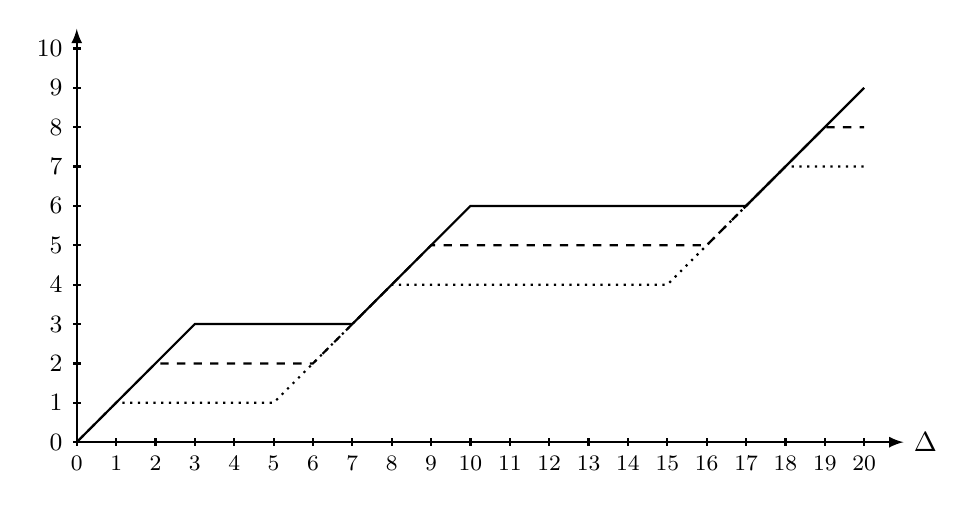
\begin{tikzpicture}[x=\ux,y=\uy, font=\sffamily,thick]  
		\draw[->] (0,0) -- coordinate (xaxis) (21,0) node[anchor=west] {$\Delta$};
		\foreach \x in {0,...,20}{
			\draw[-](\x,0.1) -- (\x,-0.1)
			node[below] {\footnotesize $\x$};
			
		}
		\draw[->] (0,0) node[anchor=east] {}-- coordinate (xaxis) (0,10.5);
		\foreach \y in {0,...,10}{
			\draw[-](0.1, \y) -- (-0.1, \y)
			node[left] {\small $\y$};
			
		}

                \draw[-,thick] (0, 0) -- (3, 3) -- (7, 3) -- (10, 6) -- (17, 6) -- (20, 9);
                \draw[-,dashed] (0 ,0) -- (2,2) -- (6, 2) -- (9, 5) -- (16, 5) -- (19, 8) -- (20, 8);
                \draw[-,dotted] (0, 0) -- (1, 1) -- (5, 1) -- (8, 4) -- (15, 4) -- (18, 7) -- (20, 7);
		\end{tikzpicture}    
  \caption{The workload function $\widehat{W}_j^0(\Delta, c_j^*)$ when $T_j=10$, $C_j=3$, and $R_j=6$. Solid line: $c_j^*$ is $3$, Dashed line: $c_j^*$ is $2$, Dotted line: $c_j^*$ is $1$.}
  \label{fig:example-lemma-workload}
\end{figure}

\noindent{\bf Physical Meaning of Theorem~\ref{theorem:general-framework}}



\begin{figure*}[t]
  \centering

		\def\ux{0.25cm}\def\uy{0.5cm} 
		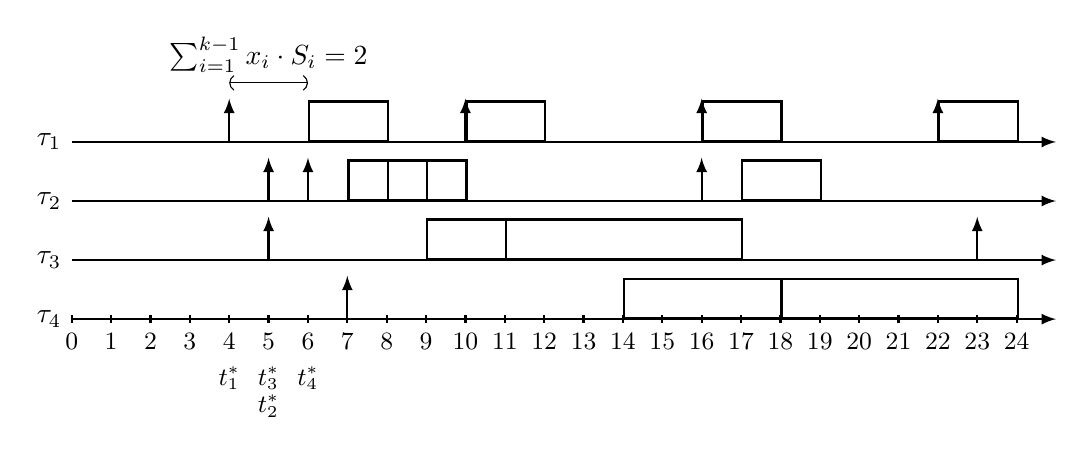
\begin{tikzpicture}[y=\uy, font=\sffamily,thick]  
		\tikzset{
			task/.style={fill=#1,  rectangle, text height=.3cm},
			task1a/.style={task=green!30},
			task1b/.style={task=green},
			task2a/.style={task=orange!30},
			task2b/.style={task=orange, minimum width=1mm},
			task3a/.style={task=pink, minimum width=1mm},
			task3b/.style={task=pink!80, minimum width=1mm},
			task4a/.style={task=cyan, minimum width=1mm},
			task4b/.style={task=cyan!50},
			task5/.style={task=blue},
			task6/.style={task=purple},
			task7/.style={minimum height=\ux,draw},
			task8/.style={minimum height=\ux,draw,thick},
			task9/.style={task=gray,minimum height=0.7cm,draw},
		}
		\tikzstyle{jobs}=[ fill=black!50];

		\begin{scope}[shift={(0,0)}]
		
		\draw[<-](2,1.1) -- (2,0);
		\draw[<-](5,1.1) -- (5,0);
		\draw[<-](8,1.1) -- (8,0);
		\draw[<-](11,1.1) -- (11,0);
		
		
		\draw[->] (0,0) node[anchor=east] {$\tau_1$}-- coordinate (xaxis) (12.5,0);

		
		\node[task7, minimum width=2*\ux,
		anchor=south west]at (3, 0){};
		\node[task7, minimum width=2*\ux,
		anchor=south west]at (5, 0){};
		\node[task7, minimum width=2*\ux,
		anchor=south west]at (8, 0){};
		\node[task7, minimum width=2*\ux,
		anchor=south west]at (11, 0){};
		\draw[(-), thin] (2, 1.5) -- (3, 1.5);
		\node[anchor=south] at (2.5, 1.5) {$\sum_{i=1}^{k-1} x_i \cdot S_i=2$};

		\end{scope}
		
		
		\begin{scope}[shift={(0,-1.5)}]
		%%timeline
		
		
		\draw[<-](2.5,1.1) -- (2.5,0);
		\draw[<-](3,1.1) -- (3,0);
		\draw[<-](8,1.1) -- (8,0);
		
		
		\node[task7, minimum width=2*\ux,
		anchor=south west] at (3.5, 0){};
		\node[task7, minimum width=2*\ux,
		anchor=south west] at (4, 0){};
		\node[task7, minimum width=2*\ux,
		anchor=south west] at (8.5, 0){};

		\draw[->] (0,0)node[anchor=east] {$\tau_2$} -- coordinate (xaxis) (12.5,0);
		
		
		\end{scope}

		\begin{scope}[shift={(0,-3)}]
		%%timeline
		
		\draw[<-](2.5,1.1) -- (2.5,0);
		\draw[<-](11.5,1.1) -- (11.5,0);
		

		\draw[->] (0,0)node[anchor=east] {$\tau_3$} -- coordinate (xaxis) (12.5,0);
		
		\node[task7, minimum width=2*\ux,
		anchor=south west]  at ( 4.5, 0){};
		\node[task7, minimum width=6*\ux,
		anchor=south west]  at ( 5.5, 0){};
		
		\end{scope}

		\begin{scope}[shift={(0,-4.5)}]
		\draw[->] (0,0) node[anchor=east] {$\tau_4$}-- coordinate (xaxis) (12.5,0);
		\draw[<-](3.5,1.1) -- (3.5,0)node[anchor=north] {$$};
				\node[task7, minimum width=4*\ux,anchor=south west]at (7, 0){};
		\node[task7, minimum width=6*\ux,anchor=south west]at (9, 0){};
		
		\foreach \x in {0,...,24}{
			\draw[-](.5*\x,0.1) -- (.5*\x,-0.1)
			node[below] {\small $\x$};
			
		}

%                \draw (10, -1.5) node {\small $f_4$};
                \draw (3, -1.5) node {\small $t_4^*$};
 %               \draw (3.5, -1.5) node {\small $t_4$};
                \draw (2.5, -1.5) node {\small $t_3^*$};
                \draw (2.5, -2.2) node {\small $t_2^*$};
                \draw (2, -1.5) node {\small $t_1^*$};
		\end{scope}
		
		\end{tikzpicture}  

\caption{An illustrative example for  the physical meaning of
  Theorem~\ref{theorem:general-framework} for Example~\ref{ex:proof_step1}.}
\label{fig:example-imaginary}  
\end{figure*}
The rationale behind Theorem \ref{theorem:general-framework} may not
be easy to be captured. A specific vector $\vec{x}$ defines how
we plan to set the release jitter for each task as follows:
\begin{itemize}
\item For task $\tau_{k-1}$, its release jitter is $R_{k-1}-C_{k-1}$
  if $x_{k-1}$ is $0$ or $S_{k-1}$ if $x_{k-1}$ is $1$.
\item For task $\tau_j$ with $j=1,2,\ldots,k-2$, its release jitter
  is
  $Q_{j+1}^{\vec{x}} + R_j-C_j$ if $x_j$ is $0$ or $Q_{j+1}^{\vec{x}}
  + S_j$ if $x_j$ is $1$.
\end{itemize}
We use the following example to explain the physical meaning
behind the setting of the release jitter of the tasks by referring to
Step 3 in the proof of Theorem~\ref{theorem:general-framework}.

  We consider Example~\ref{ex:proof_step1} when $\epsilon$ is very
  close to $0$. For such a case, $t_1^*=4,
  t_2^*=5, t_3^*=5$, and $t_4^*=6$. We consider $R_2=10$. By the above
  setting with $x_1=1, x_2=0, x_3=1$, we know that
  \begin{compactitem}
  \item the release jitter of task $\tau_3$ is $1$ with the first
    release at time $t_4^*=6$,
  \item the release jitter of task $\tau_2$ is $1+10-1=10$ with the first
    release at time $t_4^*=6$, and
  \item the release jitter of task $\tau_1$ is $1+1=2$ with the first
    release at time $t_4^*=6$.
  \end{compactitem}
  Or alternatively, we can equivalently rephrase it as follows:
  \begin{compactitem}
  \item the release jitter of task $\tau_3$ is $0$ with the first
    release at time $t_3^*=5$,
  \item the release jitter of task $\tau_2$ is $10-1=9$ with the first
    release at time $t_2^*=5$, and
  \item the release jitter of task $\tau_1$ is $0$ with the first
    release at time $t_1^*=4$.
  \end{compactitem}


  Therefore, the response time analysis in
  Lemmas~\ref{lemma:step-3-one-condition}~and~\ref{lemma:step-3-ceiling-condition}
  can be explained as follows:

  \begin{quote}\emph{A safe scenario to analyze the worst-case
      response time $R_k'$ of task $\tau_k'$ when $R_k' \leq T_k$ is
      1) to release each higher-priority task $\tau_j$ at time
      $t_j^*\equals \sum_{i=1}^{j-1} x_j S_j$ with release jitter
      $(1-x_j)(R_j-C_j)$, and 2) to execute the accumulated work only
      after time $t_k^*$, where $t_1^*$ is an arbitrary constant.}
  \end{quote}

  Figure~\ref{fig:example-imaginary} provides a schedule based on the
  above setting. Note that self-suspension does not have to be
  accounted any more after the above transformation.  Task $\tau_1$ is
  an ordinary periodic task with period $6$ with the first release at
  time $4$, and task $\tau_3$ is an ordinary periodic task with period
  $18$ with the first release at time $5$. Task $\tau_2$ is a jittered
  periodic task with period $10$ and $9$ time-unit jitter, starting at
  time $5$. Therefore, the second job of task $\tau_2$ is released at
  time $6$ in Figure~\ref{fig:example-imaginary}.

  The two idle time units are used between time $4$ and time
  $6$. These two time units are \emph{blocked} simply for accounting
  the self-suspension behavior in ${\bf T}_1$, and no job is allowed
  to be executed in this time frame.  The accumulated workload is then
  started to be executed at time $6$ and the processor does not idle
  after time $6$. Over here, we see that two jobs of task $\tau_2$ are
  executed back to back from time 7 to time 9. As shown in Figure~\ref{fig:example-imaginary}, the
  processor is busy executing the workload from time $6$ to time
  $21$. Therefore, we know that $21-6=15$ is a safe upper bound of
  $R_4$ in this example.

%The conclusion we have in the final statement of the example is that $20-7=f_k-r_k \leq  f_k-6 < 21-6$.



\begin{appProof}{of Lemma~\ref{lem:dominance_blocking}}
  In this proof, we first transform the worst-case response time analysis presented in Corollary~\ref{corollary:general-framework} in a more pessimistic analysis. We then prove that this more pessimistic version of Corollary~\ref{corollary:general-framework} provides the same solution as Eq.~\eqref{eq:TDA-suspension}, which then proves the lemma.
  
  Since $Q_i^{\vec{x}} \equals \sum_{j=i}^{k-1} S_j \times x_j$, it holds that $Q_i^{\vec{x}} \leq  Q_1^{\vec{x}}$ for $i=1,2,\ldots,k-1$. It follows that
  \begin{align*}
  & C_k + S_k + \sum_{i=1}^{k-1}\ceiling{\frac{t+Q_i^{\vec{x}}+(1-x_i)(R_i-C_i)}{T_i}} C_i\\
  \stackrel{(Q_i^{\vec{x}} \leq  Q_1^{\vec{x}})}{\leq} & C_k + S_k + \sum_{i=1}^{k-1}\ceiling{\frac{t+Q_1^{\vec{x}}+(1-x_i)(R_i-C_i)}{T_i}} C_i\\
  \stackrel{(R_i \leq D_i \leq T_i)}{\leq} & C_k + S_k + \sum_{i=1}^{k-1}\ceiling{\frac{t+Q_1^{\vec{x}}+(1-x_i)T_i}{T_i}} C_i\\
  \stackrel{(x_i \in \{0,1\})}{=} & C_k + S_k + \sum_{i=1}^{k-1} (1-x_i)C_i + \sum_{i=1}^{k-1}\ceiling{\frac{t+Q_1^{\vec{x}}}{T_i}} C_i
  \end{align*}
  
  Therefore, the smallest positive value $t$ such that  
  \begin{equation}
  \label{eq:proof_dominance_blocking}
  C_k + S_k + \sum_{i=1}^{k-1} (1-x_i)C_i + \sum_{i=1}^{k-1}\ceiling{\frac{t+Q_1^{\vec{x}}}{T_i}} C_i\leq t
  \end{equation}
  is always larger than or equal to the solution of Eq.~\eqref{eq:TDA-suspension-tighter}. 
  
  Subtituting $(t+Q_1^{\vec{x}})$ by $\theta$ in Eq.~\eqref{eq:proof_dominance_blocking}, we get that $R_k$ is upper bounded by the minimum value $(\theta-Q_1^{\vec{x}})$ greater than $0$ (and therefore by the smallest $\theta > 0$) such that 
  \begin{align}
  & C_k + S_k + \sum_{i=1}^{k-1} (1-x_i)C_i + \sum_{i=1}^{k-1}\ceiling{\frac{\theta}{T_i}}C_i\leq \theta-Q_1^{\vec{x}} \nonumber \\
  \Leftrightarrow \;\; & C_k + S_k + Q_1^{\vec{x}} + \sum_{i=1}^{k-1} (1-x_i)C_i + \sum_{i=1}^{k-1}\ceiling{\frac{\theta}{T_i}}C_i\leq \theta \nonumber \\
\Leftrightarrow \;\; & C_k + S_k + \sum_{i=1}^{k-1}(x_i S_i + (1-x_i) C_i) + \sum_{i=1}^{k-1}\ceiling{\frac{\theta}{T_i}}C_i \leq \theta \label{eq:proof_dominance_blocking_final}.
    \end{align}
    
    
    Now, consider the particular vector assignment $\vec{x}$ in which 
  \begin{equation*}
    x_i =
    \begin{cases}
      1 &\mbox{if } S_i \leq    C_i\\
      0 & \mbox{otherwise},
    \end{cases}
  \end{equation*}
  for $i=1,2,\ldots,k-1$. 
    By the definition of $B_k$ (i.e., Section~\ref{sec:suspension-blocking}), we get that 
    $$B_k = S_k + \sum_{i=1}^{k-1} \min(C_i, S_i) = S_k + \sum_{i=1}^{k-1} \left(x_i
    S_i + (1-x_i) C_i\right)$$
Eq.~\eqref{eq:proof_dominance_blocking_final} thus becomes identical to Eq.~\eqref{eq:TDA-suspension}. Therefore, if Eq.~\eqref{eq:TDA-suspension} deems a task set as being schedulable, so does Corollary~\ref{corollary:general-framework}. 
\end{appProof}

%%% Local Variables:
%%% mode: latex
%%% TeX-master: "master.tex"
%%% End:





%\setlength\bibitemsep{1pt}
%\printbibliography[maxnames=999]
%\printbibliography
%
\end{document}
% ********************************************************************
